\documentclass[a4paper]{article}

\input{MacroExtract}
\usepackage{geometry}
\geometry{hmargin=2.5cm,vmargin=1.5cm}

\title{Controlled $K$-theory for étale groupoids and applications }

\date{}
\author{ Clément Dell'Aiera}


%\usepackage{fullpage}

\begin{document}

\maketitle
This document includes extracts of my preprint, which should be published within several weeks.
\tableofcontents

\newpage

%New Version

%\section{Notations}

In this paper, $G$ will in general denote a topological groupoid, locally compact $\sigma$-compact, $A,B,D$ will be reserved for $C^*$-algebres or $G$-algebras.\\

$H$ is the separable Hilbert space. If $B$ is a $C^*$-algebra, $H_B$ is the standard right Hilbert module over $B$, i.e. \[H_B= H\otimes B=\{(b_j)\in B^\N \text{ s.t. }\sum b_j^* b_j \text{ converges in B}\}\] with the inner product $\langle b, b'\rangle = \sum b_j^* b_j'$. For any right $B$-Hilbert module $E$, $\mathcal L_B(E)$ is the $C^*$-algebra of adjoinable operators and $\mathfrak K_B(E)$ the $C^*$-algebra of compact operators of $E$ in the sense of Hilbert modules.\\

We will use the equivariant $KK$-theory of Le Gall, which are $\Z_2$-graded abelian groups $KK^G_*(A,B)$.\\

For any $G$-algebra $A$, $A\rtimes_r G$ denotes the reduced crossed-product of $A$ by $G$, $A\rtimes_{max} G$ the maximal one. 

%\begin{frame}{Motivations}

Soit $X$ un espace métrique dénombrable discret à géométrie bornée, i.e. $\sup_{x\in X} |B(x,R)|<\infty$ pour tout $R>0$. On note $H_X = l^2(X)\otimes H$ et 

\[C_R[X] = \{T\in \mathcal L(H_X) \text{ t.q. } T_{xy} \in \mathfrak K(H) \text{ et } prop(T) < R \}\]

\begin{definitionfr}[Algèbre de Roe]
\[C^*(X) = \overline{\cup_{R>0} C_R[X]} \subseteq \mathcal L(H_X).\]
\end{definitionfr}
\end{frame}

\begin{frame}
\begin{conj}[Baum-Connes coarse]
Soit $X$ un espace métrique dénombrable discret à géométrie bornée. Alors l'application d'assemblage
\[\mu_X : \varinjlim KK(C_0(P_d(X),\C) \rightarrow K(C^*(X))\]
est un isomorphisme.
\end{conj}

Soit $\Gamma$ un groupe finiment engendré par une partie symmétrique $S$. On note $|\Gamma|$ l'espace métrique obtenu en munissant $\Gamma$ de la métrique de la longueur des mots. \\

La conjecture de Baum-Connes coarse pour $|\Gamma |$ implique la conjecture de Novikov sur les hautes signatures associées à $\Gamma$. 
\end{frame}

\begin{frame}{Motivations}

\begin{thmfr}[Yu, 2010]
Soit $X$ de dimension asymptotique finie. Alors l'application d'assemblage
\[\mu_X : \varinjlim KK(C_0(P_d(X),\C) \rightarrow K(C^*(X))\]
est un isomorphisme.
\end{thmfr}

Dans la preuve : des groupes noté $QP_{\delta, r ,s, k}(X)$ et $QU_{\delta, r ,s, k}(X)$ qui approximent $K_0(C^*(X))$ et $K_1(C^*(X))$.

\end{frame}

%\section{Introduction}

This section is devoted to summarize the extent my work at the end of the second year of my PhD.\\

The aim of my subject is to study relationship between several worlds : coarse geometry, groupoids and $C^*$-algebras. The idea is to transfer ideas that were very profitable to coarse geometry into groupoids, and to try and exploit them to compute $K$-theory groups of certain groupoids. More precisely, we will consider several functors between categories which we will define later.

\[\begin{tikzcd}
\  & \textbf{Coarse} \quad (X,\mathcal E) \arrow[bend left]{dr}{G(X)} \arrow[bend right]{dl}{\beta X} \arrow{dd}{C^*X,C^*_uX}& \ \\
 \textbf{Top} \quad (Z,\mathcal T) \arrow[bend right]{dr}{C_0(Z)} & \  & \textbf{Grpds}\quad G \arrow[bend left]{dl}{C^*_r G} \\
 \ & \textbf{C}^* \quad A \arrow{d} & \ \\
\ & \textbf{KK} & \ \\
\end{tikzcd}\] 

\begin{definition}
Let $G$ be a topological groupoid, and $\mathcal E$ a family of subsets of $G$. $\mathcal E$ is said to be a coarse structure on $G$ if 
\begin{itemize}
\item[$\bullet$] if $E$ and $F$ are in $\mathcal E$, then $EF\in \mathcal E$, and $E\cup F\in \mathcal E$, $E^{-1}\in \mathcal E$
\item[$\bullet$] if $E\in \mathcal E$ and $F\subset E$, then $F\in \mathcal E$,
\item[$\bullet$] any finite subset is in $\mathcal E$ (?) and if $G^{(0)}\in \mathcal E$, $\mathcal E$ is said to be unital.
\end{itemize}
\end{definition}

\subsection{From coarse spaces to $C^*$-algebras}

\begin{definition}
A coarse space is a couple $(X,\mathcal E)$, where $X$ is a set and $\mathcal E$ a coarse structure on the pair groupoid $X\times X$. A coarse map is a map respecting the coarse structure i.e. $h : (X,\mathcal E)\rightarrow (Y,\mathcal F)$ such that $\forall F\in\mathcal F,(h\times h)^{-1}(F)\in \mathcal E$.
\end{definition}

A metric space $(X,d)$ naturally inherits a coarse structure from its bounded subsets :
\[\mathcal E_X = \{E\subset X\times X : \sup_{E} d(x,y)<\infty\}.\]

\begin{definition}
Let $(X,\mathcal E)$ be a coarse space. A $X$-module is a pair $(H_X,\phi )$ where 
\begin{itemize}
\item[$\bullet$] $H_X$ is a Hilbert space, 
\item[$\bullet$] $\phi : C_0(X)\rightarrow \mathcal L(H_X)$ is a $*$-homomorphism.
\item[$\bullet$] The module is said to be non-degenerate if $\{\phi(f)\eta : f\in C_0(X),\eta\in H_X\}$ is dense in $H_X$, and standard if no non-zero function of $C_0X)$ acts as a compact operator of $H_X$.
\end{itemize}
\end{definition}

\textbf{Examples} If $X$ is a discrete metric space with bounded geometry, $l^2(X)\otimes H$ with action by multiplication on the first factor defines a s.n.d. $X$-module.\\
If $X$ is a compact metric space endowed with a measure $\mu$ without atoms, then $L^(X,\mu)$ is a s.n.d. $X$-module.\\

\begin{definition}
Let $T\in \mathcal L(H_X, H_Y)$ be an operator.
\begin{itemize}
\item[$\bullet$] $T$ is said to be locally compact if $\phi(g)T$ and $T\phi(f)$ are compact operators for all $f\in C_0(X),g\in C_0(Y)$.
\item[$\bullet$] The support of $T$ is the complement of the set of points $(x,y)\in X\times X$ such that there exist $f_x,f_y\in C_0(X),C_0(Y)$ such that $f_x(x)\neq 0,f_{y}(y)\neq 0$ and $\phi(f_{y}) T \phi(f_x)=0$.
\item[$\bullet$] The propagation of $T$ is the smallest $E\in \mathcal E$ such that supp $T \subset E$.\textbf{ADAPTER}
\end{itemize}
\end{definition}

Let us define the Roe algebra of $X$ form a fixed s.n.d. $X$-module $H_X$. It will be shown that, up to unnatural isomorphism, it does not depend on the choice of the s.n.d. $X$-module.\\

\begin{definition}
For any $E\in \mathcal E$, define the subspace of locally compact operators with propagation $E$-controlled :
\[C_E[X,H_X] = \{T\in\mathcal L(H_X) : T \text{ is locally compact and supp }T\subset E\}.\]
The Roe algebra is the $C^*$-algebra 
\[C^*(X,H_X) = \overline{\cup_{E\in\mathcal E} C_E[X,H_X]}\]
the closure being taken with respect to the operator norm of $\mathcal L(H_X)$.
\end{definition}

\begin{prop}
Let $(X,\mathcal E),(Y,\mathcal F)$ be two coarse spaces, $H_X,H_Y$ two s.n.d. modules over $X$ and $Y$ repsectively, and $h :X\rightarrow Y$ a coarse map. Then, for any $F\in \mathcal F$, there exists an isometry $V\in \mathcal L(H_X,H_Y)$ such that
\[\text{supp }V \subset (h\times id_Y)^{-1}(E).\]
\end{prop}

\begin{dem}
Extend the representation $\phi$ to $\tilde \phi : L^\infty (X)\rightarrow \mathcal L(H_X)$. \\

Let $F\in \mathcal F$ and $\mathcal U$ be a Borel partition of $Y$ such that $\sqcup_{U\in \mathcal U} U\times U \subset F$ and every $U\in \mathcal U$ is of non-empty interior. If $\chi_A$ denotes the characteristic function of $A$, and because the modules are s.n.d., we can find an isometry \[V^{(U)} :\chi_{h^{-1}(U)}H_X \rightarrow \chi_U H_Y\] 
and by standardness $H_X =\bigoplus \chi(h^{-1}(U)) H_X$ and $H_Y =\bigoplus \chi_U H_Y$, so $V = \oplus V^{(U)}$ fits. Indeed, 
\[\text{supp }V\subset \sqcup h^{-1}(U)\times U \subset (h\times id_Y)^{-1}(F).\] 
\qed
\end{dem}

Now, if $H_X$ and $H'_X$ are two s.n.d. $X$-modules, apply the preceding lemma to the identity map to have an isometry $V: H_X\rightarrow H'_X$ which is supported as close as you want of the diagonal. This induces $Ad_V : C^*(X,H_X)\rightarrow C^*(X,H'_X)$ by $Ad_V(T) = VTV^*$, and gives our isomorphism, which is canonical in $K$-theory. \\

If we decide to fix a s.n.d. module for every coarse space, we can speak of "the" Roe algebra of $X$, and we saw that a coarse map between two coarse spaces $h : X\rightarrow Y$ induces a $*$-homomorphism $h_* : C^*(X,H_X)\rightarrow C^*(Y,H_Y)$. 

\subsection{From groupoids to $C^*$-algebras}

\subsection{From coarse spaces to groupoids}

This section gives details on he construction of the coarse groupoid from \ref{SkTuYu}.\\

Let $(X,\mathcal E)$ be a coarse space. The idea is to construct an étale groupoid $G(X)$ extending the pair groupoid $X\times X$. As a topological space, 
\[G(X)= \cup_{E\in \mathcal E} \overline{E},\]
the closure being taken in $\beta (X\times X)$, so that it is Hausdorff and locally compact. The base space is $G(X)^{(0)}=\beta X$. Now, the firt and second projections can be extended by universal property of the Stone-Cech compactification to give the source and the range map $s,r : G(X)\rightrightarrows \beta X$ respectively, as shown in this commutative diagramm :  
\[\begin{tikzcd}
X\times X \arrow{r}\arrow{d}{\iota_{X\times X}} &  X \arrow{r}{\iota_X} & \beta X \\
\beta (X\times X) \arrow[dotted]{urr} & & \\ 
\end{tikzcd}.\]

The only non trivial part is to extend the multiplication of the pair groupoid. This is done by extending the inclusion $E \rightarrow X\times X$ to $\overline{E} \rightarrow \beta X\times \beta X$. The corollary 10.31 of \ref{RoeCoarse} assures that 
\begin{lem}
The map $r\times s : \overline E \rightarrow \beta X\times \beta X$ is a topological embedding.
\end{lem}
Using this lemma, we can embed $G(X)$ in $\beta X\times \beta X$ and use the pair multiplication in this groupoid, the point being that such a multiplication $G(X)\times_{s,r} G(X) \rightarrow G(X)$ is continuous and extend the pair multiplication of $X\times X$.\\

The following proposition (Proposition $3.5$ from \ref{SkTuYu}) assures that $X\mapsto G(X)$ is a functor from uniformly locally finite coarse spaces to groupoids with generalized morphisms as arrows.\\

\begin{prop}
Let $(X,\mathcal E_X)$ and $(Y,\mathcal E_Y)$ be two coarse spaces with uniformly locally finite coarse structures, then a coarse map $h :X\rightarrow Y$ induces a generalized morphism from $G(X)$ to $G(Y)$ :
\[\begin{tikzcd}
G(X)\arrow[xshift=-0.7ex]{d}\arrow[xshift=0.7ex]{d} \ & \arrow{dl} Z \arrow{dr} & G(Y)\arrow[xshift=-0.7ex]{d}\arrow[xshift=0.7ex]{d} \\
\beta X & &\beta Y \\
\end{tikzcd}\] 
\end{prop}

We now state a result from \ref{SkTuYu} (lemma $4.4$), and give, for the reader's convenience, a more detailed proof than that of the paper.\\

\begin{prop}
Let $(X,\mathcal E)$ be a uniformly locally finite coarse space, then we have an isomorphism of $C^*$-algebras
\[C^*(X) \simeq l^\infty(X,\mathfrak K) \rtimes_r G(X).\]
\end{prop}

\begin{proof}
Let $D=l^\infty(X,\mathfrak K)$ and $G=G(X)$. The $C^*$-algebra $D\rtimes_r G$ is generated by continuous functions $f : \overline E \rightarrow D$ such that $f(g)\in D_{s(g)}\simeq \mathfrak K$ for some $E\in \mathcal E$. The crossed product is obtained as the closure in the norm operator defined by the actions of such functions by convolution on $\mathcal E = L^2(G,D)$, which defines by definition a faithful map $D\rtimes_r G \rightarrow \mathcal L(\mathcal E)$.\\

Now take the $G$-invariant ideal $J= C_0(X,\mathfrak K)$. As $D\rightarrow \mathcal M(J)$ is faithful, $\mathcal L(\mathcal E)\rightarrow \mathcal L(\mathcal E\otimes_{D} J)$ is isometric, and we obtain a faithful map by composition $D\rtimes_r G \rightarrow \mathcal L(\mathcal E\otimes_D J)$, and $\mathcal E\otimes_D J \simeq L^2(G,J)$.\\

But $C_0(X)$ acts faithfully by multiplication on $C_0(X,\mathfrak K)$, hence on $H_X=L^(G,J)$, which makes it a n.d.s. $X$-module and induces a faithful map $C^*(X,H_X) \rightarrow \mathcal L(H_X)$.\\

If $T\in C_E[X,H_X]$, define $f(g)=T_{s(g),r(g)}$ when $g\in X\times X$, and extend $f$ by continuity to get $f : \overline E \rightarrow D$, and $f(g)\in D_{s(g)}$.\\

If $f:\overline E \rightarrow D$ is a continuous function such that $f(g)\in D_{s(g)}$, define $T\in C_E[X,H_X]$ by $T\xi = f\xi$. This defines a $*$-homomorphism $D\rtimes_r G \rightarrow C^*(X,H_X)$. The previous construction shows it is surjective. But the action of $D\rtimes_r G$ on $H_X$ being faithful, it is also injective, which concludes the proof.\\
\end{proof}





































\section{Introduction}

In this article, we develop a controlled $K$-theory suited for étale groupoids, which is a generalization of the controlled or quantitative $K$-theory developed by my advisor H. Oyono-Oyono and G. Yu in \cite{OY2}. \\

One of the reasons operator $K$-theory is studied is that it is the receptacle for higher indices of elliptic differential operators. Of particular relevance to us are the following class of $C^*$-algebras :\\
\begin{itemize}
\item[$\bullet$] Roe algebras $C^*(X)$ associated to coarse spaces, whose $K$-theory encodes the higher indices of elliptic operators on noncompact complete Riemannian manifolds, 
\item[$\bullet$] Reduced crossed-products $A\rtimes_r G$ of $C^*$-algebras by an action of an étale groupoid $G$, similarly used in the context of foliations and longitudinally elliptic operators, higher indices of equivariant elliptic operators on covering spaces.\\
\end{itemize}

These examples culminate in the statement of the Baum-Connes conjecture \cite{BaumConnesHigson}, which proposes an algorithm to compute these $K$-theory groups using an assembly map, classically dentoted $\mu_{G,A} : K^{top}_*(G,A)\rightarrow K_*(A\rtimes_r G)$. The Baum-Connes conjecture asserts that $\mu_{G,A}$ is an isomorphism, and it is known to hold, for example, for groups with the Haagerup property \cite{HigsonKasparov}. This celebrated result is proved using an argument very analytical in nature, called the Dirac-Dual-Dirac method, which prevents to the author's knowledge to adapt it in other situations. For example, the injectivity of the Baum-Connes assembly map $\mu_{\Gamma,\C}$ for a discrete group implies the Novikov conjecture for higher signatures for $\Gamma$. Algebraic versions of this conjecture exists, and it is not known if the Dirac-Dual-Dirac method can be adapted in this setting.  \\

Controlled $K$-theory aims at tackling this issue, i.e. to propose other ways to prove isomorphisms of assembly maps by decomposing the object under study in simpler parts and gluying everything by Mayer-Vietoris type arguments. It is based on the celebrated proof of G. Yu \cite{Yu1} of the Novikov conjecture for groups with finite asympotitc dimension. In the course of the proof appeared some approximations of the operator $K$-theory groups. Controlled, or quantitative, $K$-theory is a nice framework to formalize this construction. It consists of a family of $\Z_2$-graded abelian groups $(K^{\varepsilon, R}(A))_{\varepsilon\in(0,\frac{1}{4},R>0}$ defined for any filtered $C^*$-algebra in the sense of \cite{OY2}. \\

The point of departure of this work is to use the coarse groupoid $G(X)$ associated to any coarse space $X$, defined in \cite{SkTuYu}, to try and understand how one can generalize the controlled $K$-theory to étale groupoids. The basic observation is the following : in $G(X)$, what encodes the propagation $R$ appearing in the controlled $K$-theory of Roe algebras are a family of compact open denoted by $\overline \Delta_R$. The crucial property is the stability of this family with respect to composition. Reversing this line of thought, one can redefine filtered $C^*$-algebras and controlled $K$-theory with respect to a groupoid using a family of compact subsets of $G$, which are thought as controlling the propagation in $G$. It turns out that, when specialized to the coarse groupoid $G(X)$, this new controlled theory gives back the results of \cite{OY2}, giving a correct generalization. We also prove controlled versions of the results of \cite{SkTuYu}, which gives a large class of examples satisfying the controlled Baum-Connes conjecture. The ultimate goal of this construction is to show that the controlled assembly maps respects stability properties, using controlled Mayer-Vietoris sequence.\\

This article is organized as follows. In the third section, we define controlled $K$-theory for étale groupoids and study some properties that will be used in the following section. Section four recall the construction of the assembly maps, both for étale groupoids and for coarse spaces. The two sections that follows are the core of the article, and detail the construction of the Controlled Coarse assembly map and the Controlled assembly map for étale groupoids. Theorem \ref{} gives a condition to relate the Controlled Baum-Connes conjecture to the classical Baum-Connes conjecture. In particular, if an étale groupoid $G$ satisfies the Baum-Connes conjecture with coefficients, it satisfies the Controlled Baum-Connes conjecture, which gives a large class of groupoids satisfying the latter. As an application, we give a strengthening of a result of \cite{OY2}, based on a result of \cite{FinnSellFibred}. The last section contains a proof of a Künneth formula in controlled $K$-theory for a class of groupoids. This class is defined as satifying a property which we could describe as being locally induced from an action of a compact grooupoid, property that we call strong properness. The main result of this section is that any étale strongly proper groupoid satisfies the restriction principle in the sense of \cite{ChabertEOY}.\\   

   

\section{Notations}

In this paper, $G$ will in general denote a topological groupoid, locally compact $\sigma$-compact, $A,B,D$ will be reserved for $C^*$-algebres or $G$-algebras.\\

$H$ is the separable Hilbert space. If $B$ is a $C^*$-algebra, $H_B$ is the standard right Hilbert module over $B$, i.e. \[H_B= H\otimes B=\{(b_j)\in B^\N \text{ s.t. }\sum b_j^* b_j \text{ converges in B}\}\] with the inner product $\langle b, b'\rangle = \sum b_j^* b_j'$. For any right $B$-Hilbert module $E$, $\mathcal L_B(E)$ is the $C^*$-algebra of adjoinable operators and $\mathfrak K_B(E)$ the $C^*$-algebra of compact operators of $E$ in the sense of Hilbert modules.\\

We will use the equivariant $KK$-theory of Le Gall, which are $\Z_2$-graded abelian groups $KK^G_*(A,B)$.\\

For any $G$-algebra $A$, $A\rtimes_r G$ denotes the reduced crossed-product of $A$ by $G$, $A\rtimes_{max} G$ the maximal one. 

\section{Controlled $K$-theory for étale groupoids}

Let $G$ be an étale groupoid. We denote $\mathcal E_G$ the set of compact subsets of $G$. Notice that if $E,E'\in \mathcal E_G$, then $E \circ E'\in\mathcal E_G$. 


\section{Assembly Maps}

In this section, all groupoids $G\rightrightarrows G^{(0)}$ are étale. 

\subsection{Proper groupoids and proper actions}

Recall that the introduction contains a survey on groupoid actions, in particular the definition of proper actions for groupoids.

%\begin{definition}
%A topological groupoid $G\rightrightarrows G^{(0)}$ is proper if the map $G\times_s G^{(0)}\rightarrow G^{(0)}\times G^{(0)}$ defined by $(g,z)\mapsto (z,gz)$ is a proper map.\\
%A $G$-space $Z$ is said to be proper if the crossed-product groupoid $Z\rtimes G$ is proper. If the space of orbits $Z/G$ is compact, $Z$ is called $G$-compact.
%\end{definition}

\begin{definition}
A $G$-space $\underline E G$ is called universal if, given any proper $G$-space $Z$, there exists a continuous $G$-equivariant map $Z\rightarrow \underline E G$.
\end{definition}

We now construct a model for universal spaces of $G$, based on J.-L.Tu's work \cite{TuBC2}. For any compact subset $K\subseteq G$, define $P_K(G)$ to be the space of probability measures $\nu $ with support contained in one and only one fiber $G^x$ for some $x\in G^{(0)}$, and such that if $g,g'\in \text{supp }(\nu)$, then $g'g^{-1}\in K$. We endow $P_K(G)$ with the weak-$*$ topology.\\

Every element $\eta$ is a finite probability measure on a fiber $G^x$, for some $x\in G^{(0)}$, hence can be written as a finite convex combination $\eta = \sum_{g\in G^{x}}\lambda_g(\eta)\delta_g$, where $\lambda_g(\eta)\in [0,1]$ for every $g$ and $\delta_g$ is the Dirac probability measure at $g\in G^x$.\\ 

Let us define a left action of $G$ on $P_K(G)$. The momentum map $p : P_K(G)\rightarrow G^{(0)}$ is the map associating to $\nu$ the only $x$ such that $\text{supp }(\nu) \subseteq G^x$. Let us show that $p$ is continuous. Let $U\subseteq G^{(0)}$ be an open set. Let $x\in U$ and $\eta\in p^{-1}(x)$. There exists an element $g\in G^x$ such that $\lambda_g(\eta) \neq 0$. Let $S\subseteq G$ be an open bisection such that $g\in S$. Up to replacing $U$ by a smaller neighborhood, we can suppose $r(S) = U$. Let $\phi : G \rightarrow [0,1]$ be a continuous function with support in $S$ such that $\phi(g) = 1$. Then $\langle \eta,\phi\rangle \neq 0$ holds. Then, $\{\eta'\in P_K(G) \text{ s.t. }\langle \eta',\phi\rangle \neq 0 \}$ is open for the weak-$*$ topology and its image through $p$ is contained in $U$. 
%Then, 
%\[p^{-1}(U) = \cup_{g\in G}\{\eta\in P_K(G) \text{ s.t. supp}( \eta ) \subseteq r^{-1}(U) \cap gK\}.\]
%As for all $g\in G$, $r^{-1}(U)\cap gK$ is compact, it is covered by a finite number of open bisections $S_1$, ... , $S_r$. Put $W_j= r^{-1}(U)\cap gK\cap S_j$ and choose open subsets $V_j\subseteq W_j$. Let us take, for each $j\in\{1,...,r\}$, a continuous function $\phi_j : G\rightarrow [0,1]$ such that $\phi$ is equal to $1$ on $V_j$ and $0$ outside of $W_j$. Then $\cup_j \{\eta\in P_K(G)\text{ s.t. } |\langle \eta, \phi_j\rangle -1|<\frac{1}{4} \}\subseteq \{\eta\in P_K(G) \text{ s.t. supp}( \eta ) \subseteq r^{-1}(U) \cap gK\}$, hence $p^{-1}(U)$ is open for the weak-$*$ topology.\\

The action is defined by left translation, i.e. for every $(g,\eta)\in G\times_{s,p}P_K(G)$ : 
\[(g.\eta)(h) = \eta(g^{-1}h)\quad \forall h\in G^{r(g)}.\]

%As the fibers are discrete, any $\nu\in P_K(G)$ can be represented as as sum $\nu = \sum_{g\in G^x} \lambda_g(\nu)\delta_g$, where $\delta_g$ is the Dirac measure at $g\in G $. The continuous functions $\lambda_g$ are called coordinate functions and satisfy $\sum_{g\in G^x} \lambda_g(\nu) =1$ for every $x\in G^{(0)}$. The action of $G$ is given by $g\lambda_h = \lambda_{g^{-1}h}$.

\begin{lem}[Tu,\cite{TuBC2}]
The action of $G$ on $P_K(G)$ is proper and cocompact.
\end{lem}  

\begin{lem}[Tu,\cite{TuBC2}]\label{Gspace}
Let $Z$ be a proper $G$-compact $G$-space. Then there exists a compact subset $K\subseteq G$ and a $G$-equivariant continuous map $Z\rightarrow P_K(G)$.
\end{lem}  

\subsection{Topological $K$-theory for groupoids}

We will use the equivariant $KK$-theory developped by Le Gall in his thesis \cite{LeGall}, which is an extension of the usual equivariant $KK$-theory of Kasparov. Recall that, if $A$ and $B$ are two $G$-algebras, elements of $KK^G(A,B)$ are homotopy classes of triple $(E,\pi,T)$ where :\\

\begin{itemize}
\item[$\bullet$] $E$ is a $G$-module, the action of $G$ being implemented by a unitary $V\in\mathcal L_{s^* B}(s^* E, r^* E)$,
\item[$\bullet$] $\pi : A\rightarrow \mathcal L_B(E)$ is a $G$-equivariant $*$-homomorphism,
\item[$\bullet$] $T\in \mathcal L_B(E)$ is an adjointable operator such that the triple satisfies the $K$-cycle conditions : $\pi(a)(T^2-T),\pi(a)(T^*-T),[\pi(a),T]$ are compact operators in $\mathfrak K(E)$, and $\pi(a)(r^*T-V s^*T V^*)$ are compact operators in $\mathfrak K_{r^* B}(r^* E)$ for all $a\in A, g\in G$.\\
\end{itemize}

\begin{definition}
Let $Y$ be a proper $G$-space and $B$ a $G$-algebra. Then the analytic $K$-homology of $Y$ with coefficients in $B$ is defined by 
\[RK^G(Y,B) = \varinjlim_{Z\subseteq Y} KK^G(C_0(Z),B), \]
the inductive limit being taken on proper $G$-compact $G$-subspaces $Z$ of $Y$. The topological $K$-theory of $G$ is defined as the analytic $K$-homology of $\underline E G$. In the litterature, the notation $K^{top}(G,B)$ is common to denote $RK^G(\underline E G,B)$.
\end{definition}

The previous lemmas ensures that the topological $K$-theory of $G$ can be computed as an inductive limit of the $K$-homology of the spaces $P_K(G)$ :
%somehow restricted when it comes to the analytic $K$-homology of any universal space $\underline E G$ :
\begin{lem}\label{Khomology} Let $B$ be a $G$-algebra. Then :
\[RK^G(\underline E G,B) = \varinjlim_{K\subseteq G \text{ compact }} KK^G(C_0(P_K(G)),B).\]
\end{lem}

\begin{dem} Let us denote by $\mathcal A$ the inductive limit 
\[\varinjlim_{K\subseteq G } KK^G(C_0(P_K(G)),B).\] 
By universal property of the inductive limit, there exists a unique homomorphism 
\[\phi : \mathcal A \rightarrow RK^G(\underline E G,B).\] 
Let $Z$ and $Z'$ be two proper $G$-compact $G$-spaces such that $Z\subseteq Z'$. By lemma \ref{Gspace}, there exist compact subsets $K$ and $K'$ of $G$ and $G$-equivariant continuous maps $h : Z\rightarrow P_K(G)$ and $h : Z'\rightarrow P_{K'}(G)$. Up to enlarge $K'$, we can suppose $h'_{|Z}$ and $ h $ are homotopic. The following diagram commutes
\[\begin{tikzcd}
KK^G(C_0(Z),B)\arrow{r}\arrow{d}{h^*} & KK^G(C_0(Z'),B)\arrow{d}{(h')^*} \\
RK^G(P_{K}(G),B)\arrow{r} & RK^G(P_{K'}(G),B) \\
\end{tikzcd},\]
hence the following  diagram :
\[\begin{tikzcd}
KK^G(C_0(Z),B)\arrow{r}\arrow{d}{\subseteq} & \mathcal A  \\
KK^G(C_0(Z'),B) \arrow{ur} &  \\
\end{tikzcd}.\]
is commutative. By universal property of the inductive limit, there exists a unique homomorphism 
\[ \psi : RK^G(\underline E G,B)\rightarrow \mathcal A.\] 
Then $\psi\circ\phi = id_A$ is obvious. As $\underline E G = \cup_K P_K(G)$, the maps $Z\rightarrow P_{K'}(G)$ and $Z\rightarrow P_{K'}(G)$ are homotopic to $Z\rightarrow \underline E G$ and $\phi\circ \psi = id$. Hence 
\[RK^G(\underline E G,B) \cong A.\]
\qed
\end{dem}

\subsection{Descent functor}

There exists a natural transformation $KK^G(A,B)\rightarrow KK(A\rtimes_r G, B\rtimes_r G)$ respecting the Kasparov product, which is called the descent functor. The same statement remains true for maximal crossed products. We recall its construction, which was first stated in \cite{LeGall}.\\
 
Let $A$ and $B$ be two $G$-algebras and $(E,\pi,T)\in E^G(A,B)$ be a $K$-cycle. Define :
\begin{itemize}
\item[$\bullet$] $E_G$ to be the $B\rtimes_r G$-Hilbert module $E\otimes_B (B\rtimes_r G)$,
\item[$\bullet$] $\pi_G = \pi\otimes_{A}id_{A\rtimes_r G} $ to be the image of $\pi:A \rightarrow \mathcal L_B(E)$ under the reduced crossed-product functor,
\item[$\bullet$] $T_G = T\otimes_{B}1$ to be the image of $T\in\mathcal L(E)$ under the reduced crossed-product functor.
\end{itemize}
Then $(E_G,\pi_G,T_G)\in E(A\rtimes_r G,B\rtimes_r G)$ and the map $(E,\pi,T)\mapsto (E_G,\pi_G,T_G) $ induces a homorphism of abelian groups
\[j_G : KK^G(A,B)\rightarrow KK(A\rtimes_r G,B\rtimes_r G)\]
satisfying $j_G(z\otimes_D z')=j_G(z)\otimes_{D\rtimes_r G} j_G(z')$ for any $z\in KK^G(A,D), z'\in KK^G(D,B)$.\\ 

\subsection{The assembly map}

If $Z$ is a proper $G$-compact $G$-space, $Z\rtimes G$ is a proper groupoid by definition, hence there exists a cutoff function $c : Z\rightarrow [0,1]$ such that $\sum_{g\in G^{p(z)}} c(zg) = 1$. The function $g\mapsto c(r(g))^{\frac{1}{2}}c(s(g))^{\frac{1}{2}} $ defines a projection in $C_0(Z)\rtimes_r G$ which we denote by $\mathcal L_Z$. If $Z=P_K(G)$, we will denote $\mathcal L_Z$ by $\mathcal L_K$. Notice that we will give a more explicit construction in this case in the following section. Indeed, for the action of $G$ on $P_K(G)$, the cutoff function can be described using well defined coordinate functions. 

\begin{definition}
The assembly map for $G$ with coefficients in $B$ is defined as the inductive limit of the maps $\mu_{G,B}^{(Z)} : KK^G(C_0(Z),B)\rightarrow K(B\rtimes_r B)$ given by
\[\mu_{G,B}^{(Z)} (z)=[\mathcal L_Z]\otimes_{C_0(Z)\rtimes G} j_G(z),\]
that is $\mu_{G,B} = \varinjlim \mu_{G,B}^{(Z)}$ (one has to check that theses maps respects the inductive systems, which they do).\\
\end{definition}

\begin{rk}\label{projection}
By lemma \ref{Khomology}, one can restrict to $Z$ of the form $P_E(G)$ for $E\subseteq G$ compact. We will denote by $\mu_{G,B}^E$ the assembly map $\mu_{G,B}^{P_E(G)}$, and $\mu_{G,B} = \varinjlim \mu_{G,B}^{E}$ still holds.
\end{rk}

%Another definition : with $Ad$...

\subsection{The Baum-Connes conjecture}

\begin{conj}[Baum-Connes conjecture]
Let $G$ be an étale groupoid, and $A$ a $G$-algebra.\\
The Baum-Connes conjecture for $G$ with coefficients in $A$ is the following claim : \\
\center{$\textbf{BC}_{G,A}$ : $\mu_{G,A}$ is an isomorphism of abelian groups.}\\
The Baum-Connes conjecture with coefficients is : for all $G$-algebras $A$, $\mu_{G,A}$ is an isomorphism of abelian groups.
\end{conj}

The conjecture was first stated for groups in \cite{BaumConnes} and in \cite{BaumConnesHigson}. The statement is a generalization of the Connes-Kasparov conjecture, which is simply, when one knows the Baum-Connes conjecture, the latter for almost connected groups (i.e. locally compact groups $G$ such that $G/G_0$ is compact, where $G_0$ is the connected component of the identity). J.-L. Tu stated the conjecture for general locally compact, $\sigma$-compact, Hausdorff groupoids with Haar systems.\cite{TuBC} \\

Here is the status of the conjecture :
\begin{itemize}
\item[$\bullet$] N. Higson and G. Kasparov proved that the conjecture with coefficients holds for groups having Haagerup property \cite{higsonkasparov}. 
\item[$\bullet$] V. Lafforgue proved the conjecture with coefficients for hyperbolic groups \cite{lafforgue2012conjecture}.
\item[$\bullet$] V. Lafforgue showed the conjecture for every semi-simple Lie group, real or $p$-adic reductive, and discrete cocompact subgroup of real rank $1$ Lie groups or of $SL(3,k)$ for any local field $k$ \cite{lafforgueT}. 
\item[$\bullet$] The Connes-Kasparov conjecture was established by J. Chabert, S. Echterhoff and R. Nest, who proved that $\mu_{G}$ is an isomorphism for every secound countable almost connected group $G$, and every group of $k$-rational points of a linear algebraic group over a local field of characteristic $0$ \cite{chabertEN}.\\
\end{itemize}

Recall that a function $h : G\rightarrow \R$ is said to be of negative type if :
\begin{itemize}
\item[$\bullet$] $h_{|G^{(0)}}=0$,
\item[$\bullet$] $h(g)=h(g^{-1})$ for all $g\in G$,
\item[$\bullet$] for all $t_i\geq 0, i=1,..,n$ such that $\sum t_i=0$ and all $g_1,...,g_n\in G$ having the same range, $\sum_i t_i t_j h(g_i^{-1} g_j )\leq 0$.
\end{itemize}
The function $h$ is said to be locally proper if, for every compact $K \subseteq G^{(0)}$, $h_{|G_K^K}$ is proper.\\

\begin{definition}
A topological groupoid $G$ is said to be a-T-menable if it satisfies one of the following equivalent property :
\begin{itemize}
\item[$\bullet$] there exists a continuous field of Hilbert spaces over $G^{(0)}$ with a proper affine action of $G$,
\item[$\bullet$] there exists a locally proper negative type function on $G$.
\end{itemize} 
\end{definition}

For groupoids, the conjecture is known to be false in full generality \cite{HigsonLaffSk}, but the following result was shown by J-L. Tu in \cite{TuThese}
\begin{thm}\label{Tu}
Let $G$ be a locally compact $\sigma$-compact Hausdorff groupoid. Then if $G$ is a-T-menable, the Baum-Connes conjecture with coefficients holds for $G$.
\end{thm}

%%%%%%%%%%%%%%%%%%%%%%%%%%%%%%%%%%%%%%%%%
\subsection{The Coarse Assembly map}
%%%%%%%%%%%%%%%%%%%%%%%%%%%%%%%%%%%%%%%%%

The construction of the coarse assembly map is very similar to the assembly map for groupoids, but relies on different functors.\\

The metric space $X$ is discrete, hence $l^2(X)$ is generated by $e_x = (\delta_{xy})_{y\in X}\in l^2(X)$. For $x,y\in X$ and $T\in \mathcal L_B(l^2(X)\otimes H_B)$, $T_{x,y}$ is defined as the unique operator in $\mathcal L_B(H_B)$ satisfying $\langle T_{xy}\xi,\eta\rangle = \langle T (e_x\otimes \xi),e_y\otimes \eta \rangle$ for all $\xi,\eta\in H_B$.\\

Recall how to define the Roe algebra $C^*(X,B)$ of a discrete metric space with bounded geometry $X$ with coefficients in an arbitrary $C^*$-algebra $B$. For $R>0$, define $C_R[X,B]$ to be the involutive subspace of operators $T\in \mathcal L_B(l^2(X)\otimes H\otimes B)$ such that $T_{xy}\in \mathfrak K_B(H\otimes B)$ and $T_{xy}=0$ as soon as $d(x,y)>R$, and $\C[X,B]= \cup_{R>0} C_R[X,B]$. 

\begin{definition}
The Roe algebra $C^*(X,B)$ is defined as the Hibert $B$-module obtained after the completion of $\C[X,B]$ with respect to the operator norm in $\mathcal L_B(l^2(X)\otimes H\otimes B)$.
\end{definition} 
%%%%%%%%%%%%%%%%%%%%%%%%%%%%%%%
This construction is functorial : any $*$-homomorphism $\phi: A\rightarrow B$ gives rise to a $*$-homomorphism $\phi_X : C^*(X,A)\rightarrow C^*(X,B)$. For the reader's convenience, we give details for the construction of $\phi\mapsto \phi_X$, which is a standard fact in Coarse Geometry.

\begin{thm}\label{Xfunctor}
Let $X$ be a discrete metric space with bounded geometry and $\phi : A\rightarrow B$ a $*$-homomorphism. Then there exists a $*$-homomorphism $\phi_X : C^*(X,A)\rightarrow C^*(X,B)$ extending $\phi$. Moreover, $\phi\mapsto \phi_X$ respects composition of $*$-homomorphisms.
\end{thm}

\begin{dem}
Recall that any $*$-morphism $\phi : A\rightarrow B$ induces, for any $A$-Hilbert module $E$, a $*$-morphism $\phi_* : \mathcal L_A(E)\rightarrow \mathcal L_B(E\otimes_A B)$. Now take $E$ to be $l^2(X)\otimes A$. Then, according to remark \ref{isometry}, $\eta\otimes a\otimes b\mapsto \eta \otimes\phi(a) b $ extends to an isometry $V\in \mathcal L_B(E\otimes_A B,l^2(X)\otimes B)$ which respects compact operators. The composition $Ad_V\circ\phi_*$ sends a compact operator $(T_{xy})_{x,y}$ to $(\phi(T_{xy}))_{x,y}$.\\

Hence, the linear map $T \mapsto V\phi_*(T)V^*$ maps $C_R[X,A]$ into $C_R[X,B]$, and so extends to a $*$-morphism $C^*(X,A)\rightarrow C^*(X,B)$. The composition property is clear from the construction.\\
\qed
\end{dem}

\begin{rk}
Notice that $\phi\rightarrow \phi_X$ can be defined in the same way for completely positive maps : for every completely positive map $\phi: A \rightarrow B$, there exists a completely positive map $\phi_X : C^*(X,A)\rightarrow C^*(X,B)$ extending $\phi$.
\end{rk}

%%%%%%%%%%%%%%%%%%%%%%%
This functoriality extends to $KK$-theory.

\begin{thm}\label{sigma} There exists a natural transformation 
\[\sigma_X : KK(A,B)\rightarrow KK(C^*(X,A),C^*(X,B))\]
which transforms the Kasparov product into composition, i.e. 
\[\sigma_X(z\otimes_D z')= \sigma_X(z')\circ \sigma_X(z) \quad \forall z\in KK(A,D),z'\in KK(D,B),\]
where the $KK$-elements $\sigma_X(z\otimes_D z')$, $ \sigma_X(z)$ and $\sigma_X(z')$ are seen as the maps they induce in $K$-theory. 
\end{thm}

\begin{rk}
This relation has to be thought as if $\sigma_X$ respects the Kasparov product. The problem is that $C^*(X,A)$ is not a separable $C^*$-algebra in general, a condition which is required for the domain of the left element in the Kasparov product. As $K(A) \cong KK(\C,A)$ for every $C^*$-algebra $A$, if $x\in K(C^*(X,A))$, $x\otimes_{C^*(X,A)}\sigma_X(z)\in KK(\C,C^*(X,B))\cong K(C^*(X,B))$ is well defined. The map $x\mapsto x\otimes_{C^*(X,A)}\sigma_X(z)$ is what we called the map induced by $\sigma_X(z)$ in $K$-theory.
\end{rk}

Let us recall the construction of $\sigma_X$. Let us first notice that $C^*(X;B\otimes\mathfrak K)\cong C^*(X,B)$. Indeed, $H$ being the separable Hilbert space, any linear isomorphism induces a $*$-isomorphism $\mathfrak K \otimes \mathfrak K \cong \mathfrak K$. An element $T\in C_R[X,B\otimes\mathfrak K]$ is then an operator such that $T_{xy}\in \mathfrak K_{B\otimes\mathfrak K}= \mathfrak K\otimes \mathfrak K \otimes B \cong \mathfrak K\otimes B$ for every $x,y\in X$. As the propagation is on the $l^2(X)$ factor, this induces the claimed isomorphism. \\

Let $(H_B,\pi,T)\in\mathbb E(A,B)$ be a $K$-cycle. Put $E = l^2(X)\otimes H\otimes A$. We can construct the internal tensor product  $E\otimes_\pi H_B$ with the help of the $*$-homomorphism $\pi : A \rightarrow \mathcal L_B(H_B)$. We also dispose of a $*$-homomorphism $\mathcal L_A(E)\rightarrow \mathcal L_B(E\otimes_\pi H_B)$. But the map 
\[(\xi\otimes a)\otimes_\pi \eta \in E\otimes_\pi H_B \mapsto \xi\otimes (\pi(a)\eta)\in l^2(X)\otimes H\otimes H_B \] %\cong l^2(X)\otimes H_B
extends to an isometry $E\otimes_\pi H_B \rightarrow l^2(X)\otimes H\otimes  H_B$. As in remark \ref{isometry}, the conjugation by this isometry sends compact operators to compact operators. Moreover, it does not alter propagation, hence $\mathcal L_A(E)\rightarrow \mathcal L_B(E\otimes_\pi H_B)\subseteq \mathcal L_B(l^2(X)\otimes H\otimes H_B)$ induces a map $\tilde \pi : C^*(X,A)\rightarrow \mathcal \mathcal M(C^*(X,B\otimes\mathfrak K))\cong \mathcal L_{C^*(X,B)}(C^*(X,B))$. Define $\tilde T$ as $1\otimes T$ acting on $l^2(X)\otimes H \otimes H_B$. Then, according to remark \ref{isometry}, the $K$-cycle relations are satisfied for $\tilde T$ and $\tilde \pi$. Hence $(l^2(X)\otimes H\otimes B,\tilde \pi,\tilde T)\in \mathbb E(C^*(X,A),C^*(X,B))$ and we put $\sigma_X([H_B,\pi,T])=[l^2(X)\otimes H\otimes B,\tilde \pi,\tilde T]\in KK(C^*(X,A),C^*(X,B))$.\\

A proof of the compatibility with Kasparov products can be found in \cite{OY3}. Notice than it can be deduced from Proposition \ref{Roe2}, where we construct a controlled morphism which induces right-multiplication by $\sigma_X(z)$ in $K$-theory and respects Kasparov products.\\ 

Let $X$ be a coarse space with bounded geometry. The Rips complex is the inductive system of finite dimensional simplicial complexes
\[P_E(X)=\{\eta\in \text{Prob}(X)\text{ s.t. supp }\eta\subseteq E\}\quad,\forall E\in \mathcal E_X,\]
endowed with the $*$-weak topology. It is an inductive system with respect to inclusion of entourages.\\
 
Let us recall the definition of the left-hand side of the coarse assembly map. The coarse homology group of $X$ with coefficients in an arbitrary $C^*$-algebra $B$ is defined as 
\[KX_*(X,B)=\varinjlim_{E\in \mathcal E_X} KK(C_0(P_E(X)),B)\]
where the limit is taken along the inductive system $\{P_E(X)\}_{E\in\mathcal E_X}$. \\

Let $E\in \mathcal E_X$. Any simplex $\eta\in P_E(X)$ can be written as a finite sum $\eta=\sum_x \lambda_x(\eta)\delta_x$ by boundedness of the geometry. Here, $\delta_x$ is the Dirac measure at $x\in X$. The functions $\lambda_x :\eta\mapsto \lambda_x(\eta)$ are continuous and satifisfy $\sum\lambda_x(\eta) = 1,\forall\eta\in P_E(X)$, so that
\[\label{V0}\tag{1} V_0\left\{\begin{array}{rcl} 
 C_0(P_E(X)) & \rightarrow 	& l^2(X)\otimes C_0(P_E(X)) 		\\ 
 f           & \mapsto 		& (\lambda_x^{\frac{1}{2}}f)_{x\in X} 
\end{array}\right.\] 
is an isometry of $C_0(P_E(X))$-modules, and $V_0V_0^*\otimes id_H$ defines a projection in $l^2(X)\otimes H\otimes C_0(P_E(X))$ with finite propagation (less than $R= \sup_E d$, because $\text{supp }(V_0 V_0^*)\subseteq E$), so a class $[\mathcal L_E]\in K_0(C^*(X,C_0(P_E(X)))$.

\begin{definition}
The coarse assembly map $\mu:KX_*(X,B)\rightarrow K_*(C^*(X,B))$ for $X$ with coefficients in $B$ is defined as 
\[\forall z\in RK(P_E(X), B), \mu_{X,B}(z)=[\mathcal L_E]\otimes_{C^*(X,C_0(P_E(X)))} \sigma_X(z).\]
\end{definition}

The coarse Baum-Connes conjecture is the following claim.

\begin{conj}[Coarse Baum-Connes conjecture]
For any coarse space $X$ with bounded geometry, the coarse assembly map $\mu_{X,\C}$ is an isomorphism.\\
\end{conj}

%%% Descent principle

One of the interesting properties of the coarse Baum-Connes conjecture is the following application to topology, which is called the descent principle. The reader is referred to J. Roe's book \cite{RoeIndex} for details. Recall that if $\Gamma$ is a finitely generated group, $|\Gamma|$ denotes the metric space obtained by choosing a set of generators and endowing $\Gamma$ with the  associated word-length metric. Also, $B\Gamma$ denotes the classifying space of $\Gamma$, which is defined in any standard textbook on algebraic topology, see \cite{May} for instance. Definitions ans statements of the Novikov conjectures can be found in \cite{ferrynovikov}. A quick reminder can be found in the introduction at \ref{Novikov}.

\begin{thm}[Descent principle]
Let $\Gamma$ be a finitely generated group such that the classifying space $B\Gamma$ has the homotopy type of a finite CW-complex. Then, the coarse Baum-Connes conjecture for $|\Gamma |$ implies the strong Novikov conjecture for $\Gamma$. 
\end{thm}

Here are some remarks about the status of the conjecture :
\begin{itemize}
\item[$\bullet$] the conjecture is known to hold for any coarse space that admits a coarse embedding into a  separable Hilbert space\cite{Yu2}.
\item[$\bullet$] counterexamples have been constructed \cite{HigsonLaffSk}.\\
%\item[$\bullet$] Let $\Gamma$ be a finitely generated group, and $|\Gamma|$ the coarse space associated to the word-length metric (any two left invariant metric on $\Gamma$ are coarsely equivalent). Then the Coarse Baum-Connes conjecture for $|\Gamma|$ implies the Novikov conjecture for higher signatures for $\Gamma$.\\
\end{itemize}

Here is another description of the coarse assembly map which will be of some interest for us.\\

Let $E\in \mathcal E_X$ be an entourage. Take a cycle $(H,\pi, T)\in E(C_0(P_E(X)), \C)$, and equip the finite dimensional simplicial complex $P_E(X)$ with a metric which restricts to the spherical metric on simplices, so that $H$ is a $P_E(X)$-module that we can suppose standard non-degenerate. Then 
\[T'=\sum \lambda_x^{\frac{1}{2}} T \lambda_x^{\frac{1}{2}} \] 
is a compact perturbation of $T$ in $\mathcal L(H)$ with bounded propagation, and is invertible modulo $C^*(P_E(X),H)$, so defines a class $[T']\in K_0(C^*(P_E(X),H))$. 
%But $P_E(X)$ and $X$ are coarsely equivalent, the barycentric map $P_E(X)\rightarrow X$ is a coarse equivalence which is covered by $V_0$, so that 
The same formula for $V_0$ than formula \ref{V0}, i.e. $V_0f = (\lambda_x^{\frac{1}{2}}f)_{x}$ defines an isometry of Hilbert spaces, still denoted $V_0$, from $l^2(P_E(X))$ to $l^2(X)\otimes l^2(P_E(X))$. Multiplication by $C_0(P_E(X))$ on the $l^2(P_E(X))$ factor endows these Hilbert spaces with a structure of $P_E(X)$-module, with respect to which the propagation of $V_0$ is bounded by $s = 2\sup_E d$. Put $V = 1\otimes V_0 $ which defines a $*$-homomorphism
\[Ad_{V} :\left\{\begin{array}{rcl} 
\mathcal L(H\otimes l^2(X)\otimes l^2(P_E(X)) ) & \rightarrow & \mathcal L(H\otimes l^2(X)\otimes l^2(P_E(X)) ) \\
T &\mapsto & VTV^* \\
\end{array}\right.\]
which sends operators of finte propagation to operators of finite propagation and respects local compactness. Hence, it induces a $*$-homomorphism $C^*(P_E(X))\rightarrow C^*(X)$ and a homomorphism
\[(Ad_{V})_* : K_*(C^*(P_E(X)))\rightarrow K_*(C^*(X)).\]
%is an isomorphism, which does only depend on the coarse class of the barycentric map.\\

With that in mind, one can show that $\mu_{X}([H,\pi,T])=(Ad_{V_0})_*[T']$.\\

Indeed, with the same notations and if $z=[H,\pi,T]\in KK(C_0(P_E(X)),\C)$, we want to compute the Kasparov product $[\mathcal L_E]\otimes \sigma_X(z)$. According to Proposition $8.7.2$ of \cite{HigsonRoe}, this is equal to the Fredholm index of $P(1\otimes T)P$ where $P=VV^*$. A simple computation shows that $V^*(1\otimes T)V=T'$ so that $P(1\otimes T)P = Ad_V(T')$, hence the equality holds.\\

The point of the article \cite{SkTuYu} is to show that the coarse assembly map is equivalent to the assembly map for the coarse groupoid $G=G(X)$ with coefficients in the $G$-algebra $l^\infty=l^\infty(X,\mathfrak K)$. \\

More precisely, let $x\in X$. Then $Z=P_{\overline E}(G)$ is a proper cocompact $G$-space with fiber $Z_x\simeq P_E(X)$, and $l^\infty_x \simeq \mathfrak K$, so that the inclusion of groupoid $\{x\}\hookrightarrow G $ induces a morphism $\iota_Z : RK^G(Z,l^\infty)\rightarrow KK(Z_x,\mathfrak K)$ which is actually an isomorphism. Recall that one can construct a $*$-isomorphism $\Psi_X: l^\infty \rtimes_r G\rightarrow C^*(X)$, and $\mu_X^{(Z_x)}\circ \iota_Z = (\Psi_X)_*\circ \mu_{G,l^\infty}^{(Z)}$ holds and respects inductive limits over $Z$ to give the following commutative diagram :
\[\begin{tikzcd}
K_*^{top}(\underline E G, l^\infty) \arrow{r}{\mu_{G,l^\infty}}\arrow{d}{\varinjlim \iota_Z} & K_*(l^\infty\rtimes_r G)\arrow{d}{(\Psi_X)_*} \\
KX_*(X)\arrow{r}{\mu_X} & K_*(C^*(X))
\end{tikzcd}\]  
with vertical arrows being isomorphism. We will give another proof of this result, based on controlled $K$-theory. Indeed, we actually prove a stronger result in theorem \ref{BCCeq}, which induces the previous result. \\

A key point is to use the correspondence between analytical properties of $G$ and coarse properties of $X$. In particular, the results of theorem \ref{propertiesXG}, combined with theorem \ref{Tu}, give examples of coarse spaces satisfying the coarse Baum-Connes conjecture and the boundary coarse Baum-Connes conjecture.

%\begin{itemize}
%\item[$\bullet$] in \cite{SkTuYu} is proved that $X$ admits a coarse embedding into Hilbert space iff $G(X)$ is a-T-menable, 
%\item[$\bullet$] in \cite{SkTuYu} is proved that $X$ has property A iff $G(X)$ is amenable, 
%\item[$\bullet$] in \cite{FinnSellFibred}, M. Finn-Sell shows that if $X$ admits a coarse fibered embedding, then $G_\partial = G(X)_{|\partial \beta X}$ is a-T-menable. 
%\end{itemize}

















\section{Controlled assembly maps for coarse spaces}

We will first construct a controlled assembly map for coarse space $(X,\mathcal E)$. In this section, $X$ will be a discrete metric space with bounded geometry, and $\mathcal E$ is the coarse structure generated by its controlled subsets. We also fix a separable Hilbert space $H$. For $R>0$, $\Delta_R$ is $\{(x,y)\in X\times X\text{ s.t. }d(x,y)<R\}$. \\

Recall first the construction of the Roe algebra of $X$ with coefficients in a $C^*$-algebra $B$, which can be found in \cite{SkTuYu}. $H_B$ denotes the standard $B$-Hilbert module $H\otimes B$. Recall that for every $x,y\in X$, and $T\in\mathcal L_B(l^2(X)\otimes H_B)$, we put $T_{xy}= \chi_y T\chi_x$ , where $\chi_x,\chi_y$ are the characteristic functions of $\{x\}$ and $\{y\}$, seen as projection operators.\\

For any positive number $R>0$, define the family of linear subspaces 
\[C_R[X,B]=\{T\in \mathcal L(l^2(X)\otimes H_B) \text{ s.t. } T_{xy}\in \mathfrak K(H_B) \text{ and }T_{xy}=0 \text{ for }(x,y)\not\in \Delta_R  \}\]
and $C^*(X,B)$ is the completion of $\cup_{R>0} C_R[X,B]$ for the operator norm in $\mathcal L(l^2(X)\otimes H_B) $. Remark that the $C^*$-algebra $C^*(X,B)$ is filtered by $\mathcal E$, and also by $\R_+^*$, seen as a coarse structure. Indeed, the composition law $R\circ R'= R+R'$ provides $\R_+^*$ with a coarse structure and $C_R[X,B] C_{R'} [X,B]\subseteq C_{R+R'}[X,B]$. For the $\mathcal E$-filtration, one can put :
\[C_E[X,B]=\{T\in \mathcal L(l^2(X)\otimes H_B) \text{ s.t. } T_{xy}\in \mathfrak K(H_B) \text{ and }T_{xy}=0 \text{ for }(x,y)\not\in E \}\quad \forall E\in\mathcal E.\]

%%%%%%%%%%%%%%%%%%%%
%For $\phi : A\rightarrow B$, we use the notation $\phi_X $ for the induced $*$-homomorphism $C^*(X,A)\rightarrow C^*(X,B)$. For the reader's convenience, we give details for its construction, which is a standard fact in Coarse Geometry.

%\begin{thm}
%Let $X$ be a discrete metric space with bounded geometry and $\phi : A\rightarrow B$ a $*$-homomorphism. Then there exists a $*$-homomorphism $\phi_X : C^*(X,A)\rightarrow C^*(X,B)$ extending $\phi$. Moreover, $\phi\mapsto \phi_X$ respects composition of $*$-homomorphisms.
%\end{thm}

%\begin{dem}
%Recall that any $*$-morphism $\phi : A\rightarrow B$ induces, for any $A$-Hilbert module $E$, a $*$-morphism $\phi_* : \mathcal L_A(E)\rightarrow \mathcal L_B(E\otimes_A B)$. Now take $E$ to be $l^2(X)\otimes A$. Then $\eta\otimes a\otimes b\mapsto \eta \otimes\phi(a) b $ extends to an isometry $V\in \mathcal L_B(E\otimes_A B,l^2(X)\otimes B)$.\\
%The linear map $T \mapsto V\phi_*(T)V^*$ maps $C_R[X,A]$ into $C_R[X,B]$, and so extends to a $*$-morphism $C^*(X,A)\rightarrow C^*(X,B)$. The composition property is clear from the construction.\\
%\qed
%\end{dem}
%%%%%%%%%%%%%%%%%%%%%%%

To construct the coarse assembly map, we will need the following proposition.

\begin{prop}\label{InverseEven}
Let $A$ be a $C^*$-algebra. The theorem \ref{Xfunctor} allows us to take the image of the exact sequence $0 \rightarrow SA \rightarrow CA \rightarrow A \rightarrow 0 $ under the functor $C^*(X,\cdot)$ to get the following filtered semi-split exact sequence 
\[0 \rightarrow C^*(X,SA) \rightarrow C^*(X,CA) \rightarrow C^*(X,A) \rightarrow 0.\] 
Let $D_{X,A} : \hat K_*(C^*(X,A))\rightarrow \hat K_*(C^*(X,SA))$ the controlled boundary morphism associated to this last extension. Then there exists a control pair $(\lambda,h)$, independent of $X$ and $A$, such that $D_{X,A}$ is $(\lambda,h)$-invertible.
\end{prop}

\begin{dem}
Recall that $0\rightarrow \mathfrak K(l^2(\N)) \rightarrow \mathcal T_0\rightarrow S\rightarrow 0 $ is the Toeplitz extension. The following diagram has exact rows and commutes
\[\begin{tikzcd} 
SC^*(X,A) \arrow{d}\arrow{r} & CC^*(X,A) \arrow{d}\arrow{r} & C^*(X,A) \arrow{d} \\ 
C^*(X,SA) \arrow{r}          & C^*(X,CA) \arrow{r}          & C^*(X,A)
\end{tikzcd}\]
so that remark \ref{rk3.8} implies that $D_{X,A} = \Psi_*\circ D_{C^*(X,A)}$. The following diagram also has exact rows and commutes
\[\begin{tikzcd} 
\mathfrak K(l^2(\N))\otimes C^*(X,A) \arrow{d}\arrow{r} & \mathcal T_0 \otimes C^*(X,A) \arrow{d}\arrow{r} & SC^*(X,A) \arrow{d} \\ 
C^*(X,\mathfrak K(l^2(\N))\otimes A) \arrow{r}          & C^*(X,\mathcal T_0 \otimes A) \arrow{r}          & C^*(X,SA)
\end{tikzcd}\]
so that remark \ref{rk3.8} implies that $D_{\mathfrak K(l^2(\N))\otimes C^*(X,A),\mathcal T_0\otimes C^*(X,A)} = D_{C^*(X,A),C^*(X,\mathcal T_0\otimes A)}\circ\Psi_*$. A simple computation shows that 
\[D_{C^*(X,A),C^*(X,\mathcal T_0\otimes A)}\circ D_{X,A} \sim D_{\mathfrak K(l^2(\N))\otimes C^*(X,A),\mathcal T_0\otimes C^*(X,A)}\circ D_{C^*(X,A)} \sim \mathcal M_{C^*(X,A)}\]
\qed
\end{dem}

\begin{rk} This result induces in $K$-theory and in $KK$-theory similar statements. Namely : 
\begin{itemize}
\item[$\bullet$] the boundary maps of the extensions $0 \rightarrow C^*(X,SA) \rightarrow C^*(X,CA) \rightarrow C^*(X,A) \rightarrow 0$ and
$0 \rightarrow\mathfrak K(l^2(\N))\otimes C^*(X,A) \rightarrow \mathcal T_0 \otimes C^*(X,A) \rightarrow SC^*(X,A) \rightarrow 0$ are inverse of each other in $K$-theory,  
\item[$\bullet$] $[\partial_{K(l^2(\N))\otimes C^*(X,A), T_0 \otimes C^*(X,A)}]$ and $[\partial_{C^*(X,SA),C^*(X,CA)}]$ are $KK$-inverse of each other.
\end{itemize}
\end{rk}

%%%%%%%%%%%%%%%%%%%%%%%%%%%%%%%%%%%%%%%%
\subsection{Controlled descent functor}
%%%%%%%%%%%%%%%%%%%%%%%%%%%%%%%%%%%%%%%%

Every $K$-cycle $z\in KK(A,B)$ can be represented as a triplet $(H_B, \pi, T)$ where :
\begin{itemize}
\item[$\bullet$]$\pi : A\rightarrow \mathcal L_B(H_B)$ is a $*$-representation of $A$ on $H_B$.
\item[$\bullet$]$T\in \mathcal L_B(H_B)$ is a self-adjoint operator.
\item[$\bullet$] $T$ and $\pi$ satisfy the $K$-cycle condition, i.e. $[T,\pi(a)]$, $\pi(a)(T^*-T)$ and $\pi(a)(T^2-id_{H_B})$ are compact operators in $\mathfrak K_B(H_B)\cong \mathfrak K \otimes B$ for all $a\in A$.\\
\end{itemize}

We first define a controlled morphism $\hat \sigma_X(z) : \hat K(A)\rightarrow \hat K(B)$ of odd degree for all $z\in KK(A,B)$, which we name the controlled Roe transform. It induces $-\otimes \sigma_X(z)$ in $K$-theory, and will be needed in the definition of the Controlled Coarse Assembly map. Recall that if $\phi : A \rightarrow B$ is a $*$-homomorphism, we denote by $\phi_X : C^*(X,A)\rightarrow C^*(X,B)$ the induced $*$-homomorphism.

\subsubsection{Odd case} %%%%%%%%%%%%%%

For $z\in KK_1(A,B)$, represented by $(H_B,\pi,T)\in E(A,B)$, define $P=(\frac{1+T}{2})\in \mathcal L_B(H_B)$ and 
%$P_X\in\mathcal L(H_{C^*(X,B)})$, and  
\[E^{(\pi,T)} = \{(a,P\pi(a)P + y) : a\in A,y\in  B\otimes \mathfrak K\} \]
which is a $C^*$-algebra such that the following sequence :
\[\begin{tikzcd}[column sep = small]0\arrow{r} & B\otimes \mathfrak K \arrow{r} & E^{(\pi,T)}\arrow{r} & A\arrow{r} & 0 \end{tikzcd}.\]
is exact and semi-split by the completely positive section $s : A\rightarrow B\otimes\mathfrak K ; a\mapsto P\pi(a)P$. Define $E_X = C^*(X,E^{(\pi,T)})$. Up to the $*$-isomomorphism $C^*(X,B\otimes\mathfrak K)\cong C^*(X,B)$, the following sequence
\[\begin{tikzcd}[column sep = small]0\arrow{r} & C^*(X,B) \arrow{r} & E_X^{(\pi,T)}\arrow{r} & C^*(X,A)\arrow{r} & 0 \end{tikzcd}.\]
is exact and semi-split by the completely positive section $s_X : C^*(X,A)\rightarrow E_X^{(\pi,T)}$.\\

\begin{prop}
The controlled boundary map $D^{(\pi,T)}=D_{C^*(X,B),E_X^{(\pi,T)}}$ of the extension $E_X^{(\pi,T)}$ only depends on the class $z$.
\end{prop}

\begin{dem}
Let $(H_B, \pi_j,T_j), j=0,1$ two $K$-cycles which are homotopic via $(H_{B[0,1]},\pi,T)$. We denote by $e_t$ the evaluation at $t\in[0,1]$ for an element of $B[0,1]$, and set $y_t=(e_t)_X(y)$ for every $y\in C^*(X,B[0,1])$. The $*$-homomorphism
\[\phi : \left\{\begin{array}{lll}E_X^{(\pi,T)} & \rightarrow & E_X^{(\pi_t,T_t)} \\ (x,y) & \mapsto & (x, y_t)\end{array}\right.\]
satisfies $\phi(C^*(X,B[0,1]))\subseteq C^*(X,B)$ and makes the following diagram commute
\[\begin{tikzcd}[column sep = small]
0\arrow{r} & C^*(X,B[0,1])\arrow{r}\arrow{d}{\phi_{|C^*(X,B[0,1])}} & E_X^{(\pi,T)} \arrow{r}\arrow{d}{\phi} & C^*(X,A)\arrow{r}\arrow{d}{=}& 0 \\
0\arrow{r} & C^*(X,B)\arrow{r} &  E_X^{(\pi_t,T_t)} \arrow{r} & C^*(X,A) \arrow{r} & 0
\end{tikzcd}.\]

According to remark \ref{rk3.8}, the following holds
\[D_{C^*(X,B),E_X^{(\pi_t,T_t)}} = \phi_* \circ D_{C^*(X,B[0,1]),E_X^{(\pi,T)}}.\]
As $id \otimes (e_t)_X$ gives a homotopy between $id\otimes (e_0)_X$ and $id\otimes (e_1)_X$, and as if two $*$-homomorphisms are homotopic, then they are equal in controlled $K$-theory, 
\[D_{C^*(X,B), E_X^{(\pi_0,T_0)}}=D_{C^*(X,B), E_X^{(\pi_1,T_1)}}\]
holds, and the boundary of the extension $E_X^{(\pi,T)}$ depends only on $z$.\\
\qed
\end{dem}

\begin{definition}
For every $z=[H_B,\pi,T]\in KK_1(A,B)$, we define the Roe transformation $\hat\sigma_X$ as 
\[\hat\sigma_X(z)= D_{C^*(X,B),E_X^{(\pi,T)}}\quad.\]
It is a $(\alpha_D,k_D)$-controlled morphism $\hat K(C^*(X,A))\rightarrow \hat K(C^*(X,B))$ of odd degree.
%, because the Morita equivalence preserves the filtration.
\end{definition}

\begin{prop}\label{Roe1}
Let $A$ and $B$ two $C^*$-algebras. There exists a control pair $(\alpha_X,k_X)$ such that for every $z\in KK_1(A,B)$, there exists a $(\alpha_X,k_X)$-controlled morphism
\[\hat\sigma_{X}(z) : \hat K_*(C^*(X,A))\rightarrow \hat K_{*+1}(C^*(X,B))\]
such that
\begin{enumerate}
\item[(i)] $\hat\sigma_X(z)$ induces right multiplication by $\sigma_{X}(z)$ in $K$-theory ;
\item[(ii)] $\hat\sigma_X$ is additive, i.e.
\[\hat\sigma_X(z+z')=\hat\sigma_X(z)+\hat\sigma_X(z').\]
\item[(iii)] For every $*$-homomorphism $f : A_1\rightarrow A_2$,
\[\hat\sigma_X(f^*(z))=\hat\sigma_X(z)\circ f_{X,*}\] for every $z\in KK_1(A_2,B)$.
\item[(iv)] For every $*$-homomorphism $g : B_1\rightarrow B_2$,
\[\hat\sigma_X(g_*(z))= g_{X,*}\circ \hat\sigma_X(z)\] for every $z\in KK_1(A,B_1)$.
\item[(v)] Let $0\rightarrow J\rightarrow A\rightarrow A/J\rightarrow 0$ be a semi-split extension of $C^*$-algebras and $[\partial_J]\in KK_1(A/J,J)$ be its boundary element. Then 
\[\hat\sigma_X([\partial_{J,A}])=D_{C^*(X,J),C^*(X,A)}.\] 
\end{enumerate}
\end{prop}

\begin{dem}
\begin{enumerate}

\item[(i)]The $K$-cycle $[\partial_{C^*(X,B),E_X^{(\pi,T)}}]\in KK_1(C^*(X,A), C^*(X,B))$ implementing the boundary of the extension $E^{(\pi,T)}$ induces the map $\sigma_X(z)$ by definition which immediately gives the first point.

\item[(ii)] If $z,z'$ are elements of $KK_1(A,B)$, represented by two $K$-cycles $(H_B,\pi_j,T_j)$, and if $(H_B,\pi,T)$ is a $K$-cycle representing the sum $z+z'$, then $E_X^{(\pi,T)}$ is naturally isomorphic to the extension sum of the $E_X^{(j)}:=E_X^{(\pi_j,T_j)}$, namely
\[\begin{tikzcd}[column sep = small]
0\arrow{r} & \mathfrak M_2( C^*(X,B)) \arrow{r} & D \arrow{r} & C^*(X,A) \arrow{r} & 0
\end{tikzcd}\]
where 
\[D=\left\{\begin{pmatrix}x_1 & k_{12}\\ k_{21} & x_2\end{pmatrix} : x_j\in E_X^{(j)} , p_1(x_1)=p_2(x_2), k_{ij}\in K(E_X^{(j)},E_X^{(i)})\right\},\]
with $p_j : E_X^{(j)}\rightarrow C^*(X,A)$ the $*$-homomorphisms of the extensions. Naturality of the controlled boundary maps \ref{rk3.8} ensures that the boundary of the sum of two extensions is the sum of the boundary of each, thus the result.

\item[(iii)] Let $z\in KK_1(A_2,B)$, represented by a cycle $(H_B,\pi,T)$. Representing $f^*(z)$ is $(H_B,f^*\pi,T)$ with $f^*\pi=\pi \circ f$. The map 
\[\phi : \left\{\begin{array}{lll} E_X^{f^*(\pi,T)} & \rightarrow & E_X^{(\pi,T)} \\
( x, P_X(f^*\pi)(x)P_X+y) & \rightarrow & ( f_X(x), P_X(f^*\pi)_X(x)P_X+y) \end{array}\right. \]
satisfies
\begin{enumerate}
\item[$\bullet$] $\phi(C^*(X,B))\subseteq C^*(X,B)$, and makes the following diagram commutes
\[\begin{tikzcd}[column sep = small]
0\arrow{r} & C^*(X,B)\arrow{r}\arrow{d}{=} & E^{f^*(\pi,T)} \arrow{r}\arrow{d}{\phi}& C^*(X,A_1)\arrow{r}\arrow{d}{f_X} & 0\\
0\arrow{r} & C^*(X,B)\arrow{r} & E^{(\pi,T)} \arrow{r}& C^*(X,A_2)\arrow{r} & 0
\end{tikzcd}.\]
\item[$\bullet$] It intertwines the sections of the two extensions.
\end{enumerate}
Remark \ref{rk3.8} ensures that \[D_{C^*(X,B), E_X^{f^*(\pi,T)} } =  D_{C^*(X,B), E_X^{(\pi,T)} }\circ f_{X,*},\] 
and the claim is clear. % from composition by $\mathcal M_{C^*(X,B)}^{-1}$.

%\item[(iv)] Let $\mathcal E = H_{B_1}\otimes_g B_2$, which is a countably generated Hilbert $B_2$-module. The homomorphism $g:B_1\rightarrow B_2$ gives rise to $g_* : \mathcal L_{B_1}(H_{B_1})\rightarrow \mathcal L_{B_2}(\mathcal E)$, which preserves compact operators : $g_*(K_{B_1})\subseteq K(\mathcal E)$. We have a similar statement for $g_X : C^*(X,B_1)\rightarrow C^*(X,B_2)$. We denote $\mathcal E_X$ the Hilbert $C^*(X,B_2)$-module $\mathcal C^*(X,E)\simeq H_{C^*(X,B_1)}\otimes_g (C^*(X,B_2))$.\\

%Let $z\in KK(A,B_1)$ be represented by the $K$-cycle $(H_{B_1},\pi,T)$. Then $(H_{B_1}\otimes_g B_2,g_*\circ\pi, g_*(T))=(\mathcal E, \tilde\pi,\tilde T)$ represents $g_*(z)$.\\

%The map $(x,y)\mapsto (x, (g_X)_*(y))$ induces $\Psi :E^{(\pi,T)}\rightarrow  E^{g_*(\pi,T)} $ such that
%\[\Psi(x,P_X \pi_X(x) P_X +y)\mapsto (x,\tilde P_X \tilde\pi_X(x) \tilde P_X+(g_X)_*(y)).\]
%Indeed, the functor $A\mapsto C^*(X,A)$ commutes with pull-back by $*$-homomorphisms, and $(g_X)*\circ\pi_X=(g_*\circ\pi)_X=\tilde \pi_X$ and $(g_X)_*(P_X) = g_*(P)_X=\tilde P_X$ so that 
%\[(g_X)_*(P_X \pi_X(x) P_X)=\tilde P_X \tilde\pi_X(x) \tilde P_X. \]
%Now, by the stabilisation lemma, we know that the countably generated Hilbert module $\mathcal C^*(X,E)$ sits as a complemented module of $H_{C^*(X,B_2)}$, and there exists a projection $p\in L(H_{C^*(X,B_2)})$ such that $pH_{C^*(X,B_2)}\simeq \mathcal E_X$ and $pK_{C^*(X,B_2)}p\simeq K(\mathcal E_X)$. Let $\psi$ be the composition $K_{C^*(X,B_1)}\rightarrow_{(g_X)_*} K(\mathcal E_X)\rightarrow K_{C^*(X,B_2)}$. In this particular case, we can give an explicit description of $\psi$. The map defined on basic tensor products $(x_j)_{j}\otimes b\mapsto (g(x_j)b)_j $ extends to an isometric embedding $\mathcal E_X \rightarrow H_{C^*(X,B_2)}$, under which $ b\theta_{e_i,e_j}$ is mapped to $g(b)\theta_{u_i,u_j}$, where $\{e_j\}$ and $\{u_j\}$ are respectively the canonical orthogonal basis of $H_{C^*(X,B_1)}$ and $H_{C^*(X,B_2)}$. This gives a commutative diagram 
%\[\begin{tikzcd}[column sep = small]
%0\arrow{r} & K_{C^*(X,B_1)}\arrow{r}\arrow{d}{\psi} & E^{(\pi,T)} \arrow{r}\arrow{d}{\Psi}& C^*(X,A)\arrow{r}\arrow{d}{=} & 0\\
%0\arrow{r} & K_{C^*(X,B_2)}\arrow{r} & E^{g_*(\pi,T)} \arrow{r}& C^*(X,A)\arrow{r} & 0
%\end{tikzcd}.\]
%and $\Psi$ intertwines the two filtered sections by the previous relation. Moreover, $\Psi_{|K_{C^*(X,B_1)}}\subseteq K_{C^*(X,B_2)}$, so that we can again apply the remark $3.7$ of \cite{OY2} to state
%\[ D_{K_{C^*(X,B_2)},E^{g_*(\pi,T)}}=\psi_*\circ D_{K_{C^*(X,B_1)},E^{(\pi,T)}},\]
%which we compose by the Morita equivalence on the left $M_{C^*(X,B_2)}^{-1}$
%\[\hat\sigma_X(g_*(z)) = M_{C^*(X,B_2)}^{-1}\circ g_{X,*}\circ D_{K_{C^*(X,B_1)},E^{(\pi,T)}}.\]
%The homomorphisms inducing the Morita equivalence make the following diagram commutes,
%\[\begin{tikzcd}C^*(X,B_1)\arrow{r}{g_X}\arrow{d} & C^*(X,B_2)\arrow{d} \\ K_{C^*(X,B_1)} \arrow{r}{\psi}& K_{C^*(X,B_2)}\end{tikzcd},\]
%and $\hat\sigma_X(g_*(z))= g_{X,*}\circ M_{C^*(X,B_1)}^{-1}\circ D_{K_{C^*(X,B_1)},E^{(\pi,T)}}=g_{X,*}\circ \hat\sigma(z)$.\\

%%%%%%%%%%%%%%%%%%%%%%%%
%%%  NOUVELLE PREUVE  %%
%%%%%%%%%%%%%%%%%%%%%%%%

\item[(iv)]
Let $z \in KK(A,B_1)$ be represented by the $K$-cycle $(H_{B_1},\pi,T)$. Let $V\in \mathcal L_{B_2}(H_{B_1}\otimes_g B_2)$ be the isometry of remark \ref{isometry}. According to Lemma \ref{isometryKK}, 
\[g_*(z)=[H_{B_1}\otimes_g B_2, \pi\otimes_g 1, T\otimes_g 1]\in KK^G(A,B_2)\] 
is also represented by $[H_{B_2}, \pi',T' ]$ where $\pi' = Ad_{V}\circ (\pi\otimes_g 1)$ and $T' = V(T\otimes_g 1)V^* +1-VV^*$. Let $\psi$ be given by the composition $Ad_{V_X}\circ g_X$.\\
The map $\Psi :(x,y)\mapsto (x, \psi(y))$ defines a $*$-homomorphism $E_X^{(\pi,T)} \rightarrow E_X^{(\pi',T')}$ such that 
\[\Psi(x,P_X\pi_X(x)P_X +y)= (x, P'_X  \pi_X'(a)P'_X + \psi(y)) ).\] 
Indeed, the functor $C^*(X,-)$ commutes with pull-back by $*$-homomorphisms, and $Ad_{V_X}\circ g_X\circ\pi_X= (Ad_V\circ g \circ \pi)_X = \pi'_X$ and $\psi(P_X)= V_X (P_X\otimes_{g_X} 1)V^*_X = (V(P\otimes_g 1 ) V^*)_X = (P')_X$ so that 
\[\psi(P_X \pi_X(x) P_X)=P'_X \pi'_X(x) P'_X. \]
This gives a commutative diagram 
\[\begin{tikzcd}[column sep = small]
0\arrow{r} & C^*(X,B_1)\arrow{r}\arrow{d}{\psi} & E^{(\pi,T)} \arrow{r}\arrow{d}{\Psi}& C^*(X,A)\arrow{r}\arrow{d}{=} & 0\\
0\arrow{r} & C^*(X,B_2)\arrow{r} & E^{(\pi',T')} \arrow{r}& C^*(X,A)\arrow{r} & 0
\end{tikzcd}.\]
and $\Psi$ intertwines the two filtered sections by the previous relation. Moreover, $\Psi (C^*(X,B_1))\subseteq C^*(X,B_2)$, so that we can again apply the remark \ref{rk3.8} to state
\[ D_{C^*(X,B_2),E_X^{(\pi',T')}}=\psi_*\circ D_{C^*(X,B_1),E_X^{(\pi,T)}}\ .\]
%which we compose by the Morita equivalence on the left $M_{C^*(X,B_2)}^{-1}$
Under the identification $C^*(X,B\otimes\mathfrak K) \cong C^*(X,B)$, $\psi = g_X$, hence
\[\hat\sigma_X(g_*(z)) = g_{X,*}\circ D_{C^*(X,B_1),E_X^{(\pi,T)}}.\]
The homomorphisms inducing the Morita equivalence make the following diagram commutes,
\[\begin{tikzcd}C^*(X,B_1)\arrow{r}{g_X}\arrow{d} & C^*(X,B_2)\arrow{d} \\ K_{C^*(X,B_1) } \arrow{r}{\psi}& K_{C^*(X,B_2)}\end{tikzcd},\]
and $\sigma_X(g_*(z))= g_{X,*}\circ M_{C^*(X,B_1)}^{-1}\circ D_{K_{C^*(X,B_1)},E^{(\pi,T)}}=g_{X,*}\circ \sigma_X(z)$.\\

\item[(v)] Let $q:A\rightarrow A/J$ be the quotient map and $(H_J, \pi, T)$ be a cycle representing $[\partial_{J,A}]$ and $P=\frac{1+T}{2}$. Consider the following commutative diagram :
\[\begin{tikzcd}[column sep = small]
0\arrow{r} &J\arrow{r}\arrow{d} & A \arrow{r}\arrow{d}{\phi}& A/J\arrow{r}\arrow{d}{=} & 0\\
0\arrow{r} & J\otimes \mathfrak K\arrow{r} & E^{(\pi,T)} \arrow{r}& A/J\arrow{r} & 0
\end{tikzcd},\]
where $\phi(a) = (q(a),P\pi(q(a))P)$ and $J\rightarrow J\otimes \mathfrak K; j\mapsto j\otimes e;$ with $e$ a rank one projection. We apply $C^*(X,-)$ to get the commutative diagram
\[\begin{tikzcd}[column sep = small]
0\arrow{r} & C^*(X,J)\arrow{r}\arrow{d} & C^*(X,A) \arrow{r}\arrow{d}{\phi_X}& C^*(X,A/J)\arrow{r}\arrow{d}{=} & 0\\
0\arrow{r} & C^*(X,J)\arrow{r} & E_X^{(\pi,T)} \arrow{r}& C^*(X,A/J)\arrow{r} & 0
\end{tikzcd},\]
where the lines are semi-split filtered and exact. Remark \ref{rk3.8} applies and $D_{J,A} = D_{C^*(X,J),E_X^{(\pi,T)}}$.\\
%where the first vertical arrow is the canonical mapping that induces the Morita equivalence. \\
\end{enumerate}
\qed
\end{dem}

\subsubsection{Even case} %%%%%%%%%%%%%%%

We can now define $\hat\sigma_X$ for even $K$-cycles. Let $A$ and $B$ be two $C^*$-algebras and $z\in KK(A,B)$. Recall that $[\partial_{SB}]\in KK_1(B,SB)$ is the $K$-cycle implementing the boundary of the extension $0\rightarrow SB\rightarrow CB\rightarrow B\rightarrow 0$, and $[\partial]\in KK_1(\C,S)$ is the Bott generator. Recall from proposition \ref{InverseEven} that $D_{X,A}$  and $D_{ C^*(X,A),C^*(X,\mathcal T_0\otimes A) }$ are controlled inverse of each other. We will denote $D_{ C^*(X,A),C^*(X,\mathcal T_0\otimes A) }$ by $T_{X,A}$.\\

As $z\otimes_B [\partial_{SB}]$ is an odd $K$-cycle, we can define
\[\hat\sigma_X(z):= T_{X,B}\circ \hat\sigma_X(z\otimes[\partial_{SB}]).\] 

%Here $\tau_D$ refers to the $(\alpha_\tau,k_\tau)$-controlled map $\hat K (A_1\otimes D )\rightarrow \hat K(A_2\otimes D)$, that H. Oyono-Oyono and G. Yu constructed in \cite{OY2} for any $C^*$-algebras $D,A_1,A_2$ and $z\in KK_*(A_1,A_2)$. It enjoys many natural properties, and induces right multiplication by $\tau_D(z)\in KK(A_1\otimes D,A_2\otimes D)$ in $K$-theory. We can see that, if we set $\alpha_J=\alpha_\tau \alpha_D$ and $k_J=k_\tau * k_D$, $\hat\sigma(z)$ is $(\alpha_X,k_X)$-controlled.\\

\begin{prop}\label{Roe2}
Let $A$ and $B$ two $C^*$-algebras. For every $z\in KK_*(A,B)$, there exists a control pair $(\alpha_X,k_X)$ and a $(\alpha_X,k_X)$-controlled morphism
\[\hat\sigma_X(z) : \hat K(C^*(X,A))\rightarrow \hat K(C^*(X,B))\]
of the same degree as $z$, such that
\begin{enumerate}
\item[(i)] $\hat\sigma_X(z)$ induces right multiplication by $\sigma_X(z)$ in $K$-theory ;
\item[(ii)] $\hat\sigma_X$ is additive, i.e.
\[\hat\sigma_X(z+z')=\hat\sigma_X(z)+\hat\sigma_X(z').\]
\item[(iii)] For every $*$-homomorphism $f : A_1\rightarrow A_2$,
\[\hat\sigma_X(f^*(z))=\hat\sigma_X(z)\circ f_{X,*}\] for all $z\in KK_*(A_2,B)$.
\item[(iv)] For every $*$-homomorphism $g : B_1\rightarrow B_2$,
\[\hat\sigma_X(g_*(z))= g_{X,*}\circ \hat\sigma_X(z)\] for all $z\in KK_*(A,B_1)$.
\item[(v)] $\hat\sigma_X([id_A]) \sim_{(\alpha_X,k_X)} id_{\hat K(C^*(X,A))}$
\end{enumerate}
\end{prop}

\begin{dem} The work is already done for odd $KK$-elements. Let $z\in KK_0(A,B)$.
\begin{enumerate}
\item[(i)] Proposition \ref{Roe1} ensures that $\hat \sigma_X(z\otimes [\partial_{SB}])$ induces right multiplication by $\sigma_X(z\otimes [\partial_{SB}])$ in $K$-theory. Proposition \ref{InverseEven} implies that $T_{X,B}$ induces multiplication by $[\partial_{C^*(X,B),C^*(X,B\otimes\mathcal T_0)}]^{-1}$ in $K$-theory. Hence, according to theorem \ref{sigma}, their composition induces $ \sigma_X([\partial_{A,\mathcal T_0 \otimes  A}]^{-1})\circ\sigma_X([\partial_{SB}])\circ\sigma_X(z)$ where we identify $KK$-elements with the maps they induce in $K$-theory. But this element is just $\sigma_X(z)$, because  $\sigma_X([\partial_{A,\mathcal T_0 \otimes  A}]^{-1})\circ\sigma_X([\partial_{SB}])= id_{K(C^*(X,B))}$.
\item[(ii)] This is clear by \ref{Roe1}.
\item[(iii)] It is a consequence of the previous proposition \ref{Roe1}, and of the equality $f^*(x)\otimes_D y = f^*(x\otimes_D y)$ for every $*$-homomorphism $f : A'\rightarrow A$ and for every $x\in KK(A,D),y\in KK(D,B)$.
\item[(iv)] By naturality of the boundary element, we have $g_*(z)\otimes_{B_2} [\partial_{SB_2}] = z\otimes_{B_1} g^{*}[\partial _{SB_2}] = (Sg)_{*}(z\otimes_{B_1} [\partial _{SB_1}])$, hence, by proposition \ref{Roe1}, 
\[\hat\sigma_X(g_*(z)) = T_{X,B_2}\circ ((Sg)_X)_* \circ \hat\sigma_{X}(z\otimes_{B_1} [\partial_{SB_1}]).\]
Controlled boundaries are natural, hence $T_{X,B_2}\circ ((Sg)_X)_* = (g_X)_* \circ T_{X,B_1}$, and $\hat\sigma_X(g_*(z)) =(g_X)_* \circ \hat\sigma_X(z)$.
\item[(v)] The same argument we used for the first point concludes.
\end{enumerate}
\qed
\end{dem}

We now show that the Roe transform respects in a quantitative way the Kasparov product. Let us recall the following result from \cite{lafforgue2002k}. It states that every $KK$-element comes from the product of an element coming from a $*$-homomorphism and an element coming from the inverse in $KK$-theory of a $*$-homomorphism. Recall property $(d)$ from \ref{propertyD}, which is just this statement for groupoids. In other words, when the groupoid is a locally compact group, property $d$ is property $2$.

\begin{lem}[\cite{lafforgue2002k}, lemma $1.6.11$] Let $A$ and $B$ be two $C^*$-algebras and $z\in KK(A,B)$. Then, there exists a $C^*$-algebra $A_1$, an element $\alpha \in KK(A,A_1)$ and $*$-homomorphims $\theta : A_1 \rightarrow A$ and $\eta : A_1 \rightarrow B$ such that
$\theta^*(\alpha) = id_{A_1}$, $\theta_*(\alpha) = id_{A}$ and $\theta^*(z) = \eta$.
\end{lem}

\begin{prop} There exists a control pair $(\alpha_R,k_R)$ such that for every $C^*$-algebras $A$, $B$ and $C$, and every $z\in KK(A,B),z'\in KK(B,C)$, the controlled equality
\[\hat\sigma_X(z\otimes_B z') \sim_{\alpha_R,k_R} \hat\sigma_X(z')\circ \hat\sigma_X(z)\]
holds.
\end{prop}

\begin{dem}
The previous lemma reduces the proof to the special case of $\alpha\in KK(A,B)$ being the inverse of a $*$-homomorphism $\theta : B\rightarrow A$ in $KK$-theory : $\alpha\otimes_B [\theta]=1_A$. Let $z\in KK(B,C)$ :
\[\begin{array}{rcl}
\hat\sigma_X (\alpha\otimes z) & \sim_{\alpha_J^2,k_J*k_J} &  \hat\sigma_X (\alpha\otimes z)\circ \hat\sigma_X (\alpha\otimes [\theta]) \\
			& \sim & \hat\sigma_X (\alpha\otimes z)\circ \hat\sigma_X (\theta_*(\alpha))\\
			& \sim & \hat\sigma_X (\alpha\otimes z)\circ \theta_{X,*}\circ \hat\sigma_X (\alpha)\\
			& \sim & \hat\sigma_X (\theta^*(\alpha\otimes z))\circ \hat\sigma_X (\alpha)\\
			& \sim & \hat\sigma_X (z)\circ \hat\sigma_X (\alpha) \\
\end{array}\] 
because $\theta^*(\alpha\otimes z)=\theta^*(\alpha)\otimes z=1\otimes z =z$. The control on the propagation of the first line follows from remark $2.5$ of \cite{OY2} and point $(v)$, the other lines are equal by points $(iii)$ and $(iv)$, hence $(\alpha_R,k_R)$ can be taken to be $(2 \alpha_X^{4},( k_X)^{*2})$.
\qed
\end{dem}

\subsection{Controlled coarse assembly maps}

%If $(X,\mathcal E_X)$ is a coarse space, and $E\in\mathcal E_X$ a controlled subset, any simplex $\eta$ of the Rips complex $P_E(X) = \{m \in Prob(X)\text{ s.t. supp }m \subseteq E\}$ can be written as $\eta = \sum_{x\in X} \lambda_x(\eta) \delta_x$, where $\delta_x$ si the Dirac probability at $x$, and $\lambda_x : P_E(X)\rightarrow [0,1]$ is a continuous function. Set :
Let $E\in\mathcal E$ be a controlled subset. Then any simplex $\eta$ of the Rips complex $P_E(X)$ can be written as $\eta = \sum_{x\in X} \lambda_x(\eta) \delta_x$, where $\delta_x$ si the Dirac probability at $x$, and $\lambda_x : P_E(X)\rightarrow [0,1]$ is a continuous function. Set :
\[ P_E : \left\{\begin{array}{rcl} X \times X & \rightarrow & C_0(P_E(X))\\  (x,y) & \mapsto & \lambda_x^{\frac{1}{2}}\lambda_y^{\frac{1}{2}}\end{array}\right. \]  
As $\sum_{x\in X} \lambda_x =1$, $P_E$ is a projection of $\mathfrak K(l^2(X)) \otimes C_0(P_E(X))$ of controlled support : $\text{supp }P_E\subseteq E$. Hence $P_E$ defines a class $[P_E,0]_{\varepsilon, E'}\in K_0^{\varepsilon, E'} (C^*(X,C_0(P_E(X)))$ for any $\varepsilon\in (0,\frac{1}{4})$ and any $E'\in\mathcal E$ satisfying $E\subseteq E'$.\\

For every $C^*$-algebra $B$ and every controlled subsets $E,E'\in\mathcal E$ such that $E\subseteq E'$, the canonical inclusion $P_E(X)\hookrightarrow P_{E'}(X)$ induces a $*$-homomorphism $q_E^{E'} : C_0(P_{E'}(X))\rightarrow C_0(P_{E}(X))$, hence a map $(q_E^{E'})^* : KK(C_0(P_E(X)),B)\rightarrow KK(C_0(P_{E'}(X)),B)$ in $KK$-theory and a map $(q_E^{E'})_* : K(C_0(P_{E'}(X)))\rightarrow K(C_0(P_{E}(X)))$ in $K$-theory. The family of projections $P_E$ are compatible with the morphims $q_E^{E'}$, i.e. $((q_E^{E'})_X)_*[P_{E'},0]_{\varepsilon,E'} = [P_{E},0]_{\varepsilon,E}$, for every $\varepsilon\in (0,\frac{1}{4})$.
%Moreover, the inclusion being an isometry, we have a map $K(C^*(P_E(X), B)) \rightarrow K(C^*(P_E(X), B))$, still denoted $q_E^{E'}$.

\begin{definition}
Let $B$ a $C^*$-algebra, $\varepsilon\in (0,\frac{1}{4})$ and $E,F\in\mathcal E_X$ controlled subsets such that $k_X(\varepsilon).E\subseteq F$. The controlled coarse assembly map $\hat\mu_{X,B}=(\mu_{X,B}^{\varepsilon,E,F})_{\varepsilon,E}$ is defined as the family of maps
\[\hat\mu_{X,B}^{\varepsilon, E,F} :\left\{\begin{array}{rcl} KK(C_0(P_E(X)),B) & \rightarrow & K^{\varepsilon, F}(C^*(X,B)) \\
					z & \mapsto & \iota_{\alpha_X \varepsilon',k_X(\varepsilon').F'}^{\varepsilon,F}\circ\hat\sigma_X(z)[P_{E},0]_{\varepsilon', F'}\end{array}\right.\]
where $\varepsilon'$ and $F'$ satisfy :
\begin{itemize}
\item[$\bullet$] $\varepsilon\in (0,\frac{1}{4})$ such that $\alpha_X \varepsilon'\leq \varepsilon$,
\item[$\bullet$] and $F'\in\mathcal E$ such that $E\subseteq F'$ and $k_X(\varepsilon).F'\subseteq F$.
\end{itemize}
%are chosen not to exceed $\varepsilon$ and $E$ when composed with the propagation of the controlled morphisms. 
\end{definition}

\begin{rk} The controlled coarse assembly map is compatible with the structure morphisms $q_E^{E'}$. Indeed, for every $E,E'\in \mathcal E$ such that $E\subseteq E'$, by proposition \ref{Roe2}, 
\[\hat\sigma_X((q_E^{E'})^*(z))[P_{E'},0]_{\varepsilon,E'}  = \hat\sigma_X(z)\circ ((q_E^{E'})_X)_*[P_E',0]_{\varepsilon,E'}= \hat\sigma_X(z)[P_E,0]_{\varepsilon,E}.\] 
Hence $\hat\mu_{X,B}^{\varepsilon,E,F}\circ(q_E^{E'})^* =\hat\mu_{X,B}^{\varepsilon,E',F}$.
\end{rk}

\begin{rk} The controlled coarse assembly map is also compatible with the structure morphisms $\iota_{\varepsilon,E}^{\varepsilon',E'}$, i.e. $\iota_{\varepsilon,F}^{\varepsilon',F'}\circ\hat\mu_{X,B}^{\varepsilon,E,F} =\hat\mu_{X,B}^{\varepsilon',E,F'}$. Hence, the controlled coarse assembly map $\hat \mu_{X,B}$ induces the coarse assembly map $\mu_{X,B}$ in $K$-theory.
\end{rk}

\begin{rk}
This assembly map is defined for the usual Roe algebra of $X$, but could be defined for any "nice" completion of the algebraic Roe algebra $\cup_{E\in \mathcal E_X} C_E[X]$. In particular, we can define an assembly map with values in the controlled $K$-theory of the maximal Roe algebra $C_{max}
^*(X)$.\end{rk}

 


































\section{Controlled assembly maps for coarse spaces}

\section{Controlled assembly maps for étale groupoids}

\subsection{Kasparov transform}

Let $A$ and $B$ be two $\G$-$C^*$-algebras, and $H$ a separable Hilbert space, $l^2(\Z)$ for instance, and $H_\G= H\otimes L^2(\G,\lambda)$. The standard Hilbert module over $B$ is denoted by $H_B=H_\G\otimes B$, and $K_B$ is the algebra of compact operators for $H_B$, i.e. $K(H)\otimes L^2(\G,\lambda)\otimes B$. \\

Every $K$-cycle $z\in KK^G(A,B)$ can be represented as a triplet $(H_B, \pi, T)$ where :
\begin{itemize}
\item[$\bullet$]$\pi : A\rightarrow \mathcal L_B(H_B)$ is a $*$-representation of $A$ on $H_B$.
\item[$\bullet$]$T\in \mathcal L_B(H_B)$ is a self-adjoint operator.
\item[$\bullet$] $T$ and $\pi$ verify the $K$-cycle condition, i.e. $[T,\pi(a)]$, $\pi(a)(T^2-id_{H_B})$ and $\pi(a)(g.T-T)$ are compact operator over $H_B$ for all $a\in A, g\in \G$.\\
\end{itemize}

Set $T_\G= T\otimes id_{B\rtimes \G}\in \mathcal L_{B\rtimes \G}(H_B\otimes (B\rtimes \G))\simeq \mathcal L_{B\rtimes \G}(H_{B\rtimes\G})$, and $\pi_G: A\rtimes \G v\rightarrow L_{B\rtimes \G}(H_{B\rtimes\G})$. Then, according to Le Gall \cite{LeGall}, $(H_{B\rtimes\G, \pi_\G, T_\G})$ represents the $K$-cycle $j_\G(z)\in KK(A\rtimes \G,B\rtimes \G)$. Let us construct a controlled morphism associated to $z$,
\[J_\G(z) : \hat K(A\rtimes \G)\rightarrow \hat K(B\rtimes\G), \]
which induces right multiplication by $j_\G(z)$ in $K$-theory.\\

\subsubsection{Odd case}

Let us first do the work for $z\in KK_1^\G(A,B)$. Let $(H_B,\pi,T)$ be a $K$-cycle representing $z$. Set $P=\frac{1+T}{2}$ and $P_\G=P\otimes id_{B\rtimes \G}$. We define
\[E^{(\pi,T)}=\{(x,P_G\pi_G(x)P_\G + y) : x\in A\rtimes \G, y\in K_{B\rtimes\G}\}\]
a $C^*$-algebra which is filtered by
\[E_R^{(\pi,T)}=\{(x,P_G\pi_G(x)P_\G + y) : x\in (A\rtimes \G)_R, y\in K\otimes (B\rtimes\G)_R\}\]
which gives us a filtered extension
\[\begin{tikzcd}[column sep = small]
0\arrow{r} & K_{B\rtimes_r\G}\arrow{r} & E^{(\pi,T)} \arrow{r} & A\rtimes_r \G \arrow{r}& 0
\end{tikzcd}\]
and semi split by  $s :\left\{\begin{array}{lll}A\rtimes_r \G & \rightarrow & E^{(\pi,T)} \\ x & \mapsto & (x, P_\G \pi_\G(x)P_\G)\end{array}\right.$.\\

Let us show that the controlled boundary map of this extension does not depend on the representant chosen, but only on the class $z$.\\
Let $(H_B, \pi_j,T_j), j=0,1$ two $K$-cycles which are homotopic via $(H_{B[0,1]},\pi,T)$. We denote $e_t$ the evaluation at $t\in[0,1]$ for an element of $B[0,1]$, and set $y_t=e_t(y)$ for such a $y$. The $*$-morphism
\[\phi : \left\{\begin{array}{lll}E^{(\pi,T)} & \rightarrow & E^{(\pi_t,T_t)} \\ (x,y) & \mapsto & (x, y_t)\end{array}\right.\]
satisfies $\phi(K_{B[0,1] \rtimes_r \G})\subset K_{B \rtimes_r \G}$ and makes the following diagram commute
\[\begin{tikzcd}[column sep = small]
0\arrow{r} & K_{B[0,1] \rtimes_r \G}\arrow{r}\arrow{d}{\phi_{|K_{B[0,1] \rtimes_r \G}}} & E^{(\pi,T)} \arrow{r}\arrow{d}{\phi} & A\rtimes_r \G \arrow{r}\arrow{d}{=}& 0 \\
0\arrow{r} & K_{B \rtimes_r \G}\arrow{r} &  E^{(\pi_t,T_t)} \arrow{r} & A\rtimes_r \G \arrow{r} & 0
\end{tikzcd}.\]

According to \cite{OY2}, remark $3.7.$, the following holds
\[D_{K_{B\rtimes_r\G,E^{(\pi_t,T_t)}}} = \phi_* \circ D_{K_{B[0,1]\rtimes_r\G},E^{(\pi,T)}}.\]
As $id \otimes e_t$ gives a homotopy between $id\otimes e_0$ and $id\otimes e_1$, and as if two $*$-morphisms are homotopic, then they are equal in controlled $K$-theory, 
\[D_{K_{B\rtimes_r \G}, E^{(\pi_0,T_0)}}=D_{K_{B\rtimes_r \G}, E^{(\pi_1,T_1)}}\]
holds, and the boundary of the extension $E^{(\pi,T)}$ depends only on $z$.\\

\begin{definition}
The controlled Kasparov transform of an element $z\in KK_1^\G(A,B)$ is defined as the compostion
\[J_{red,\G}(z)=\mathcal M_{B\rtimes_r \G}^{-1}\circ D_{K_{B\rtimes_r \G}, E^{(\pi,T)}}.\]
\end{definition}

As the boundary map is a $(\alpha_D,k_D)$-controlled morphism and the Morita equivalence preserves the filtration, $J_{red,\G(z)}$ is  $(\alpha_D,k_D)$-controlled. 

\begin{prop}\label{Kasparov1}
Let $A$ and $B$ two $\G$-$C^*$-algebras. There exists a control pair $(\alpha_J,k_J)$ such that for every $z\in KK^\G_1(A,B)$, there exists a $(\alpha_J,k_J)$-controlled morphism
\[J_{red,\G}(z) : \hat K_*(A\rtimes_r \G)\rightarrow \hat K_{*+1}(B\rtimes_r \G)\]
such that
\begin{enumerate}
\item[(i)] $J_{red,\G}(z)$ induces right multiplication by $j_{red,\G}(z)$ in $K$-theory ;
\item[(ii)] $J_{red,\G}$ is additive, i.e.
\[J_{red,\G}(z+z')=J_{red,\G}(z)+J_{red,\G}(z').\]
\item[(iii)] For every $\G$-morphism $f : A_1\rightarrow A_2$,
\[J_{red,\G}(f^*(z))=J_{red,\G}(z)\circ f_{\G,red,*}\] for all $z\in KK_1^G(A_2,B)$.
\item[(iv)] For every $\G$-morphism $g : B_1\rightarrow B_2$,
\[J_{red,\G}(g_*(z))= g_{\G,red,*}\circ J_{red,\G}(z)\] for all $z\in KK_1^G(A,B_1)$.
\item[(v)] Let $0\rightarrow J\rightarrow A\rightarrow A/J\rightarrow 0$ be a semi-split equivariant extension of $\G$-algebras and $[\partial_J]\in KK_1^\G(A/J,J)$ be its boundary element. Then 
\[J_\G([\partial_J])=D_{J\rtimes_r G,A\rtimes_r\G}.\] 
\end{enumerate}
\end{prop}

\begin{dem}
\begin{enumerate}

\item[(i)]The $K$-cycle $[\partial_{K_{B\rtimes_r \G},E^{(\pi,T)}}]\in KK_1(A\rtimes_r \G, B\rtimes_r \G)$ implementing the boundary of the extension $E^{(\pi,T)}$ induces the map $j_{red,\G}$ by definition, and modulo Morita equivalence, which immediately gives the first point.

\item[(ii)] If $z,z'$ are elements of $KK_1^G(A,B)$, represented by two $K$-cycles $(H_B,\pi_j,T_j)$, and if $(H_B,\pi,T)$ is a $K$-cycle representing the sum $z+z'$, then $E^{(\pi,T)}$ is naturally isomorphic to the extension sum of the $E_j:=E^{(\pi_j,T_j)}$, namely
\[\begin{tikzcd}[column sep = small]
0\arrow{r} & K_{B\rtimes_r \G} \arrow{r} & D \arrow{r} & A\rtimes_r \G \arrow{r} & 0
\end{tikzcd}\]
where 
\[D=\left\{\begin{pmatrix}x_1 & k_{12}\\ k_{21} & x_2\end{pmatrix} : x_j\in E_j , p_1(x_1)=p_2(x_2), k_{ij}\in K(E_j,E_i)\right\}.\]
Naturality of the controlled boundary maps \cite{OY2} ensures that the boundary of the sum of two extensions is the sum of the boundary of each, thus the result.
\item[(iii)] Let $z\in KK_1^\G(A_2,B)$, represented by a cycle $(H_B,\pi,T)$. Representing $f^*(z)$ is $(H_B,f^*\pi,T)$ with off course $f^*\pi=\pi \circ f$. The map 
\[\phi : \left\{\begin{array}{lll} E^{f^*(\pi,T)} & \rightarrow & E^{(\pi,T)} \\
( x, P_\G(f^*\pi)(x)P_\G+y) & \rightarrow & ( f_\G(x), P_\G(f^*\pi)(x)P_\G+y) \end{array}\right. \]
satisfies
\begin{enumerate}
\item[$\bullet$] $\phi(K_{B\rtimes_r \G})\subset K_{B\rtimes_r \G}$, and makes the following diagram commute
\[\begin{tikzcd}[column sep = small]
0\arrow{r} & K_{B\rtimes_r \G}\arrow{r}\arrow{d}{=} & E^{f^*(\pi,T)} \arrow{r}\arrow{d}{\phi}& A_1\rtimes_r \G\arrow{r}\arrow{d}{f_\G} & 0\\
0\arrow{r} & K_{B\rtimes_r \G}\arrow{r} & E^{(\pi,T)} \arrow{r}& A_2\rtimes_r \G\arrow{r} & 0
\end{tikzcd}.\]
\item[$\bullet$] It intertwines the sections of the two extensions.
\end{enumerate}
Remark $3.7$ of \cite{OY2} assures that \[D_{K_{B\rtimes_r \G}, E^{f^*(\pi,T)} } =  D_{K_{B\rtimes_r \G}, E^{(\pi,T)} }\circ f_{\G,*}\], and the claim is clear from composition by $\mathcal M_{B\rtimes_r \G}^{-1}$.

\item[(iv)] Let $\mathcal E = H_{B_1}\otimes_g B_2$, which is a countably generated Hilbert $B_2$-module. The homomorphism $g:B_1\rightarrow B_2$ gives rise to $g_* : \mathcal L_{B_1}(H_{B_1})\rightarrow \mathcal L_{B_2}(\mathcal E)$, which preserves compact operators : $g_*(K_{B_1})\subset K(\mathcal E)$. We have a similar statement for $g_G : B_1\rtimes\G\rightarrow B_2\rtimes\G$. We denote $\mathcal E_G$ the Hilbert $B_2\rtimes\G$-module $\mathcal E\rtimes\G\simeq H_{B_1\rtimes \G}\otimes_g (B_2\rtimes \G)$.\\

Let $z\in KK^\G(A,B_1)$ be represented by the $K$-cycle $(H_{B_1},\pi,T)$. Then $(H_{B_1}\otimes_g B_2,g_*\circ\pi, g_*(T))=(\mathcal E, \tilde\pi,\tilde T)$ represents $g_*(z)$.\\

The map $(x,y)\mapsto (x, (g_G)_*(y))$ induces $\Psi :E^{(\pi,T)}\rightarrow  E^{g_*(\pi,T)} $ such that
\[\Psi(x,P_G \pi_G(x) P_G +y)\mapsto (x,\tilde P_G \tilde\pi_G(x) \tilde P_G+(g_G)_*(y)).\]
Indeed, the crossed-product functor commutes with pull-back by $\G$-morphisms, and $(g_G)*\circ\pi_G=(g_*\circ\pi)_G=\tilde \pi_G$ and $(g_G)_*(P_G) = g_*(P)_G=\tilde P_G$ so that 
\[(g_G)_*(P_G \pi_G(x) P_G)=\tilde P_G \tilde\pi_G(x) \tilde P_G. \]
Now, by the stabilisation lemma of Le Gall \cite{LeGall}, we know that the countably generated Hilbert module $\mathcal E_G$ sits as a complemented module of $H_{B_2\rtimes\G}$, and there exists a projection $p\in L(H_{B_2\rtimes\G})$ such that $pH_{B_2\rtimes\G}\simeq \mathcal E_\G$ and $pK_{B_2\rtimes\G}p\simeq K(\mathcal E_G)$. Let $\psi$ be the composition $K_{B_1\rtimes \G}\rightarrow_{(g_G)_*} K(\mathcal E_\G)\rightarrow K_{B_2\rtimes \G}$. In this particular case, we can give an explicit description of $\psi$. The map defined on basic tensor products $(x_j)_{j}\otimes b\mapsto (g(x_j)b)_j $ extends to an isometric embedding $\mathcal E_\G \rightarrow H_{B_2\rtimes \G}$, under which $ b\theta_{e_i,e_j}$ is mapped to $g(b)\theta_{u_i,u_j}$, where $\{e_j\}$ and $\{u_j\}$ are respectively the canonical orthogonal basis of $H_{B_1 \rtimes\G}$ and $H_{B_2 \rtimes\G}$. This gives a commutative diagram 
\[\begin{tikzcd}[column sep = small]
0\arrow{r} & K_{B_1\rtimes \G}\arrow{r}\arrow{d}{\psi} & E^{(\pi,T)} \arrow{r}\arrow{d}{\Psi}& A\rtimes_r \G\arrow{r}\arrow{d}{=} & 0\\
0\arrow{r} & K_{B_2\rtimes \G}\arrow{r} & E^{g_*(\pi,T)} \arrow{r}& A\rtimes \G\arrow{r} & 0
\end{tikzcd}.\]
and $\Psi$ intertwines the two filtered sections by the previous relation. Moreover, $\Psi_{|K_{B_1\rtimes \G}}\subset K_{B_2\rtimes\G}$, so that we can again apply the remark $3.7$ of \cite{OY2} to state
\[ D_{K_{B_2\rtimes \G},E^{g_*(\pi,T)}}=\psi_*\circ D_{K_{B_1\rtimes \G},E^{(\pi,T)}},\]
which we compose by the Morita equivalence on the left $M_{B_2\rtimes\G}^{-1}$
\[J_\G(g_*(z)) = M_{B_2\rtimes\G}^{-1}\circ g_{G,*}\circ D_{K_{B_1\rtimes \G},E^{(\pi,T)}}.\]
The homomorphisms inducing the Morita equivalence make the following diagram commutes,
\[\begin{tikzcd}B_1\rtimes\G\arrow{r}{g_\G}\arrow{d} & B_2\rtimes \G\arrow{d} \\ K_{B_1\rtimes\G } \arrow{r}{\psi}& K_{B_2\rtimes\G }\end{tikzcd},\]
and $J_\G(g_*(z))= g_{G,*}\circ M_{B_1\rtimes\G}^{-1}\circ D_{K_{B_1\rtimes \G},E^{(\pi,T)}}=g_{G,*}\circ J_\G(z)$.\\
\item[(v)] Let $q:A\rightarrow A/J$ be the quotient map and $(H_J, \pi, T)$ be a cycle representing $[\partial_J]$. Then we apply remark $3.7$ of \cite{OY2} to the commutative diagram
\[\begin{tikzcd}[column sep = small]
0\arrow{r} & J\rtimes \G\arrow{r}\arrow{d} & A\rtimes \G \arrow{r}\arrow{d}{s\circ q_\G}& A/J\rtimes_r \G\arrow{r}\arrow{d}{=} & 0\\
0\arrow{r} & K_{J\rtimes \G}\arrow{r} & E^{(\pi,T)} \arrow{r}& A/J\rtimes \G\arrow{r} & 0
\end{tikzcd},\]
where the first vertical arrow is the canonical mapping that induces the Morita equivalence. \\
\qed
\end{enumerate}
\end{dem}

\subsubsection{Even case}

We can now define $J_\G$ for even $K$-cycles. Let $A$ and $B$ be two $\G$-algebras. Let $[\partial_{SB}]\in KK_1(B,SB)$ be the $K$-cycle implementing the boundary of the extension $0\rightarrow SB\rightarrow CB\rightarrow B\rightarrow 0$, and $[\partial]\in KK_1(\C,S)$ be the Bott generator. As $z\otimes_B [\partial_{SB}]$ is an odd $K$-cycle, we can define
\[J_\G(z):= \tau_{B\rtimes \G}([\partial]^{-1})\circ J_\G(z\otimes[\partial_{SB}]).\] 

Here $\tau_D$ refers to the $(\alpha_\tau,k_\tau)$-controlled map $\hat K (A_1\otimes D )\rightarrow \hat K(A_2\otimes D)$, that H. Oyono-Oyono and G. Yu constructed in \cite{OY2} for any $C^*$-algebras $D,A_1,A_2$ and $z\in KK_*(A_1,A_2)$. It enjoys many natural properties, and induces right multiplication by $\tau_D(z)\in KK(A_1\otimes D,A_2\otimes D)$ in $K$-theory. We can see that, if we set $\alpha_J=\alpha_\tau \alpha_D$ and $k_J=k_\tau * k_D$, $J_\G(z)$ is $(\alpha_J,k_J)$-controlled.\\

\begin{prop}
Let $A$ and $B$ two $\G$-$C^*$-algebras. For every $z\in KK^\G_*(A,B)$, there exists a control pair $(\alpha_J,k_J)$ and a $(\alpha_J,k_J)$-controlled morphism
\[J_{red,\G}(z) : \hat K(A\rtimes_r \G)\rightarrow \hat K(B\rtimes_r \G)\]
of the same degree as $z$, such that
\begin{enumerate}
\item[(i)] $J_{red,\G}(z)$ induces right multiplication by $j_{red,\G}(z)$ in $K$-theory ;
\item[(ii)] $J_{red,\G}$ is additive, i.e.
\[J_{red,\G}(z+z')=J_{red,\G}(z)+J_{red,\G}(z').\]
\item[(iii)] For every $\G$-morphism $f : A_1\rightarrow A_2$,
\[J_{red,\G}(f^*(z))=J_{red,\G}(z)\circ f_{\G,red,*}\] for all $z\in KK_*^G(A_2,B)$.
\item[(iv)] For every $\G$-morphism $g : B_1\rightarrow B_2$,
\[J_{red,\G}(g_*(z))= g_{\G,red,*}\circ J_{red,\G}(z)\] for all $z\in KK_*^G(A,B_1)$.
\item[(v)] $J_G([id_A]) \sim_{(\alpha_J,k_J)} id_{\hat K(A\rtimes \G)}$
\end{enumerate}
\end{prop}

\begin{dem}
The point $(iii)$ is a consequence of the previous proposition \ref{Kasparov1}, and of the equality $f^*(x)\otimes y = f^*(x\otimes y)$.\\
\qed
\end{dem}

We now show that the controlled Kasparov transform respects in a quantitative way the Kasparov product.

\begin{prop} There exists a control pair $(\alpha_K,k_K)$ such that for every $\G$-$C^*$-algebra $A$, $B$ and $C$, and every $z\in KK^\G(A,B),z'\in KK^\G(B,C)$, the controlled equality
\[J_\G(z\otimes_B z') \sim_{\alpha_K,k_K} J_\G(z')\circ J_\G(z)\]
holds.
\end{prop}
\begin{dem}
We will use the following fact : there exists a positive integer $d$ such that every cycle $z\in KK^\G(A,B)$ has decomposition property $(d)$. For more details, we send to the appendice of the article of V. Lafforgue \cite{LaffOY} where H. Oyono-Oyono shows that claim. We just need to know that $z$ satisfies the decomposition property $(d)$ if there exist $d+1$ $\G$-$C^*$-algebras $A_j$  and $d$ cycles $\alpha_j\in KK^\G(A_{j-1},A_j), j=1,d$ such that $A_0=A$, $A_d=B$ and each $\alpha_j$ is either coming from a $*$-morphism $A_{j-1}\rightarrow A_j$, or there is a $*$-morphism $\theta_j: A_j\rightarrow A_{j-1}$ such that $\alpha_j \otimes_{A_j} [\theta_j]=1$ in $KK^G(A_{j-1},A_{j-1})$.\\

This property reduces the proof to the special case of $\alpha$ being the inverse of a morphism in $KK^\G$-theory : $\alpha\otimes[\theta]=1$, then :
\[\begin{array}{rcl}
J_\G (\alpha\otimes z) & \sim_{\alpha_J^2,k_J*k_J} &  J_\G(\alpha\otimes z)\circ J_\G(\alpha\otimes [\theta]) \\
			& \sim & J_\G(\alpha\otimes z)\circ J_\G(\theta_*(\alpha))\\
			& \sim & J_\G(\alpha\otimes z)\circ \theta_{\G,*}\circ J_\G(\alpha)\\
			& \sim & J_\G(\theta^*(\alpha\otimes z))\circ J_\G(\alpha)\\
			& \sim & J_\G(z)\circ J_\G(\alpha) \\
\end{array}\] 
because $\theta^*(\alpha\otimes z)=\theta^*(\alpha)\otimes z=1\otimes z =z$. The control on the propagation of the first line follows from remark $2.5$ of \cite{OY2} and point $(v)$, the other lines are equal by points $(iii)$ and $(iv)$. As $d$ is uniform for all locally compact groupoids with Haar systems, a simple induction concludes, and $(\alpha_K,k_K)$ can be taken to be $(d \alpha_J^{2d},( k_J*k_J)^{*d})$.
\qed
\end{dem}
\subsection{Quantitative assembly maps}

Following the article of J.-L. Tu \cite{TuBC}, we recall that a locally compact, $\sigma$-compact and Hausdorff groupoid $G$, endowed with a Haar system $\lambda$, is said to be proper if there exists a cut-off function $c:G^{(0)}\rightarrow \R_+$ continuous such that 
\begin{itemize}
\item[$\bullet$] for all compact subset $K$ of $G^{(0)}$, $\text{supp }c\cap s(G^K)$ is compact,
\item[$\bullet$] $\int_{G^x}c(s(g))d\lambda^x(g)=1,\forall x \in G^{(0)}$.
\end{itemize}
If moreover $G^{(0)}/G$ is also compact, reducing the first condition to "$\text{supp }c$ compact", then $g\mapsto \sqrt{c(r(g))c(s(g))}$ defines a projection in $C_c(G)$ for convolution, which gives an element $[\mathcal L_G] \in K_0(C^*G)$.\\

Now when $X$ is a locally compact space which is $\G$-proper and $\G$-compact, the groupoid $X\rtimes\G$ is proper with a compact orbit base space ($X/\G$ is compact). We can then define $[\mathcal L_X]\in K_0(C_0(X)\rtimes_r \G)$ as the class of the projector for $G=X\rtimes\G$.


\begin{frame}{Künneth}
Pour toutes $C^*$-algèbres $A$ et $B$, on définit
\[\alpha_{A,B} : K_*(A)\otimes K_*(B)\rightarrow K_*(A\otimes B) \quad ; \quad (x,y)\mapsto x\otimes   \tau_A(y).\]

\begin{definitionfr}
Une $C^*$-algèbre $A$ satisfait la formule de Künneth si, pour toute $C^*$-algèbre $B$ telle que $K_*(B)$ soit libre, $\alpha_{A,B}$ est un isomorphisme.
\end{definitionfr}

Si $A$ satisfait la formule de Künneth, alors, pour toute $C^*$-algèbre $B$, la suite suivante
\[0  \rightarrow K_*(A)\otimes K_*(B) \rightarrow K_*(A\otimes B)  \rightarrow Tor(K_*(A),K_*(B)) \rightarrow 0\]
est exacte.

\end{frame}

\begin{frame}{Künneth}
Si $A$ est $\mathcal E$-filtrée, $A\otimes B$ est $\mathcal E$-filtrée par $\{A_E\otimes B\}_E$. On définit le morphisme contrôllé  
\[\hat\alpha_{A,B} : \hat K_*(A)\otimes K_*(B)\rightarrow \hat K_*(A\otimes B) \quad ; \quad (x,y)\mapsto \hat\tau_A(y)(x),\]
qui induit $\alpha_{A,B}$ en $K$-théorie.\\
\end{frame}

\begin{frame}{Künneth}
Le morphisme contrôllé $\alpha_{A,B}$ est dit :
\begin{itemize}
 
\item[$\bullet$] quasi-injectif s'il existe $\lambda \geq 1$ tel que, pour tout $\varepsilon\in (0,\frac{1}{4\alpha_\tau \lambda})$ et $F\in\mathcal E$, il existe $F'\in\mathcal E$, et $F\subseteq F'$, tels que: 
\[\forall x\in K^{\varepsilon,F}(A)\otimes K(B)\text{ such that }\alpha_{A,B}^{\varepsilon,F}(x)=0 \text{ then }(\iota_{\varepsilon,F}^{\lambda\varepsilon,F'}\otimes id) (x) = 0.\] 

\item[$\bullet$] quasi-surjectif s'il existe $\lambda \geq 1$ tel que, pour tout $\varepsilon \in (0,\frac{1}{4\alpha_\tau})$ et $F\in\mathcal E$, il existe $F'\in\mathcal E$, $F\subseteq h_{\tau,\lambda\varepsilon}.F'$, tels que:
\[ \forall y\in K^{\varepsilon,F}(A\otimes B), \exists x\in K^{\lambda\varepsilon, F'}(A)\otimes K(B) \text{ such that }
\alpha^{\lambda\varepsilon,F'}_{A,B}(x)=\iota_{\varepsilon,F}^{\alpha\lambda\varepsilon,h_{\tau, \lambda\varepsilon}.F'}(y).\] 

\end{itemize}
\end{frame}

\begin{frame}{Künneth}
\begin{definitionfr}
Une $C^*$-algèbre $\mathcal E$-filtrée $A$ satisfait la formule de Künneth quantitative s'il existe $\lambda \geq 1$ tel que, pour toute $C^*$-algèbre $B$ telle que $K_*(B)$ soit libre, $\hat\alpha_{A,B}$ est quasi-injective et quasi-surjectif. 
\end{definitionfr}
\end{frame}

\begin{frame}{Künneth}
\begin{thmfr}
Soit $G$ un groupoïde étale de la classe $\mathcal C$, et soient $E\in\mathcal E$ un ensemble contrôlé de $G$ et $P_E(G)$ le complexe de Rips associé. Si, pour tout sous-groupoïde compact ouvert $H$ de $G$ et tout $H$-espace $V$ tel que l'application moment $p : V\rightarrow H^{(0)}$ soit localement injective, $\alpha_{Res_H^G(A),B}^{H,V}$ est un isomorphisme, alors $\alpha_{A,B}^{G,P_E(G)}$ est un isomorphisme pour toute $C^*$-algèbre $B$ telle que $K_*(B)$ est un groupe abélien libre.\\
\end{thmfr}
\end{frame}

\begin{frame}{Künneth}
\begin{thmfr}
Soit $G$ un groupoïde $\sigma$-compact étale et $A$ une $G$-algèbre. Si 
\begin{itemize}
\item[$\bullet$] $G$ vérifie la conjecture de Baum-Connes à coefficients,
\item[$\bullet$] $G$ est un groupoïde fortement propre,
\item[$\bullet$] pour tout sous-groupoïde compact $H$ de $G$ et tout $H$-espace $V$ telle que l'application moment $p : V\rightarrow H^{(0)}$ soit localement injective, $\alpha_{Res_H^G(A),B}^{G,V}$ est un isomorphisme.
\end{itemize} 
Alors $A\rtimes_r G$ vérifie la formule de Künneth contrôlée.
\end{thmfr}
\end{frame}

\begin{frame}{Künneth}
\end{frame}

\begin{frame}{Künneth}
\end{frame}


%Old Version
\newpage
%We say that a $\mathrm{C}^*$-algebra $A$ satisfies the \textit{Künneth formula} if for all $\mathrm{C}^*$-algebras $B$ there exists a canonical short exact sequence
	\begin{equation} \label{KunnethSequence}	
0\longrightarrow \K_*(A)\otimes \K_*(B)\stackrel{\alpha}{\longrightarrow}\K_*(A\otimes B)\stackrel{\beta}{\longrightarrow}\mathrm{Tor}(\K_*(A),\K_*(B))\longrightarrow 0,
	\end{equation}
	where $A\otimes B$ denotes the minimal tensor product of $A$ and $B$ and $\K_*$ denotes $\ZZ /2\ZZ$-graded $\K$-theory. \\

The Künneth formula is known to hold for every $C^*$-algebras in the bootstrap class $\mathcal B$, from the results of Rosenberg and Schochet \cite{RosenbergKunneth}. Recall that $\mathcal B$ is the smallest class of separable nuclear $C^*$-algebras such that:
\begin{itemize}
\item[$\bullet$] $\C \in \mathcal B$,
\item[$\bullet$] $\mathcal B$ is closed under countable inductive limits,  
\item[$\bullet$] $\mathcal B$ is closed under $KK$-equivalence,
\item[$\bullet$] if $0 \rightarrow I \rightarrow A \rightarrow A/I \rightarrow 0$ is a short exact sequence of $C^*$-algebras and two of these are in $\mathcal B$, so is the third. 
\end{itemize}
In the groupoid setting, J-L. Tu proved (\cite{TuThese}, lemma $10.6$) that every a-T-menable groupoid $G$ has its reduced $C^*$-algebra $C^*_r(G)$ in $\mathcal B$. Some $C^*$-algebras are known not to be in $\mathcal B$ and to satisfy the Künneth formula, such as reduced $C^*$-algebras of lattices in $Sp(n,1)$. Indeed, if $A\in \mathcal B$, then $A$ is $KK$-equivalent to a commutative $C^*$-algebra (see \cite{blackadar}, corollary $20.10.3$). Moreover, a result of Skandalis (\cite{SkandalisNotion}) shows that if $\Gamma$ is an infinite hyperbolic property T group, then $C^*_r(\Gamma)$ is not $K$-nuclear. In particular, it cannot be KK-equivalent to a commutative $C^*$-algebra (a more recent reference for this result is theorem $6.2.1$ of the notes of N. Higson and E. Guentner \cite{HigsonGuentnerNotes}) so that $C^*_r(\Gamma)$ is not in $\mathcal B$. But corollary $0.2$ of J. Chabert, S. Echterhoff and H. Oyono-Oyono \cite{ChabertEOY} together with V. Lafforgue's result \cite{lafforgue2012conjecture} that hyperbolic groups satisfy the Baum-Connes conjecture with coefficients imply that $C^*_r(\Gamma)$ satisfies the Künneth formula.\\

The goal of this work is to extend the results of \cite{ChabertEOY} to the setting of \'etale groupoids. Let us first recall these results, before stating definitions we will need about groupoid crossed-products. The result we are trying to extend is the following:

\begin{thm}[\cite{ChabertEOY}, Th. 0.1 and Cor. 0.2] Let $G$ be a locally compact group and $A$ a $G$-algebra such that:
\begin{itemize}
\item[$\bullet$] $G$ satisfies the Baum-Connes conjecture with coefficients in all $C^*$-algebras $A\otimes B$ for all $C^*$-algebras $B$ with trivial $G$-action,
\item[$\bullet$] for every $C^*$-algebra $B$, considered as a $G$-algebra with trivial action, and every compact subgroup $K$ of $G$, $A\rtimes_r K$ satisfies the Künneth formula.
\end{itemize}
Then $A\rtimes_r G$ satisfies the Künneth formula.
\end{thm}

In this paper we study the question of when $A$ satisfies the Künneth formula for the case that $A=C\rtimes_r G$ is a (reduced) crossed product, where $G$ is an ample groupoid and $C$ is a $G$-algebra.
	We follow the strategy of \cite{CEO} and compare existence of the sequence \ref{KunnethSequence} to the existence of a canonical exact sequence

		\begin{equation}\label{MixedSequence}
		0\rightarrow \K_*^{\mathrm{top}}(G;C)\otimes\K_*(B)\stackrel{\alpha_G}{\rightarrow}\K_*^{\mathrm{top}}(G;C\otimes B)\stackrel{\beta_G}{\rightarrow}\mathrm{Tor}(\K_*^{\mathrm{top}}(G;C),\K_*(B))\rightarrow 0\\
		\end{equation}

	Here $\K_*^{\mathrm{top}}(G;C)$ denotes the topological $\K$-theory of $G$ with coefficient $C$. The link between the sequences \ref{MixedSequence} and \ref{KunnethSequence} is given by the Baum-Connes assembly map $\mu_C:\K_*^{\mathrm{top}}(G;C)\rightarrow K_*(C\rtimes_r G)$.
	Let $\mathcal{N}_G$ denote the class of all separable exact $G$-algebras $C$ for which the canonical exact sequence \ref{MixedSequence} exists. We show that whenever $C$ is in $\mathcal{N_G}$ and $G$ satisfies the Baum-Connes conjecture with coefficients in $C\otimes B$ for all separable $\mathrm{C}^*$-algebras $B$ with respect to the trivial action on $B$, then $A=C\rtimes_r G$ satisfies the Künneth formula.
	We then use the machinery of Going-Down functors to show, that the class $\mathcal{N}_G$ is non-empty, and in fact fairly large by proving the following results.
	\begin{thmx}(see Theorem \ref{Theorem:Kunneth} and Corollary \ref{Cor:Kunneth})
		Let $G$ be an ample groupoid and $A$ a separable and exact $G$-algebra. Suppose that $A_{\mid K}\rtimes K$ satisfies the (ordinary) Künneth formula for all compact open subgroupoids $K\subseteq G$. Then $A\in \mathcal{N}_G$. In particular, if the fibre $A_x$ is type I for all $x\in G^{(0)}$, then $A\in \mathcal{N}_G$.
	\end{thmx}
	
	As an immediate consequence of this and Proposition \ref{Prop:BCandKunneth} we get the following.
	\begin{corx}(see Corollary \ref{Corollary:Kunneth})
		Let $G$ be an ample groupoid and $A$ a separable and exact $G$-algebra. Suppose that $A_{\mid K}\rtimes K$ satisfies the (ordinary) Künneth formula for all compact open subgroupoids $K\subseteq G$. Suppose further that $G$ satisfies the Baum-Connes conjecture for $A\otimes B$ for every $\mathrm{C}^*$-algebra $B$ (with $G$ acting trivially on $B$).
		Then $A\rtimes_r G$ satisfies the Künneth formula. 
	\end{corx}
	
	We also show that the class $\mathcal{N}_G$ enjoys many stability properties. Among these we prove that $\mathcal{N}_G$ is stable under taking inductive limits. To prove this we show that the topological $\K$-theory is continuous with respect to the coefficient algebra, which constitutes another application of the Going-Down principle and is inspired by \cite[§7]{MR1836047}:
	\begin{thmx}(see Theorem \ref{Theorem:Continuity of top. K-theory})
		Let $G$ be an ample groupoid and $(A_n,\varphi_n)_n$ an inductive sequence of $G$-algebras. If we let $A=\lim A_n$, then the maps $\psi_{n,*}:\K_*^{\mathrm{top}}(G;A_n)\rightarrow \K_*^{\mathrm{top}}(G;A)$ induced by the canonical maps $\psi_n:A_n\rightarrow A$, give rise to an isomorphism
		$$\lim_{n\rightarrow\infty}\K_*^{\mathrm{top}}(G;A_n)\cong \K_*^{\mathrm{top}}(G;A).$$
	\end{thmx}
	An immediate consequence is the following permanence property for the Baum-Connes conjecture:
	\begin{corx}(see Corollary \ref{Cor:InductiveLimit})
		Let $G$ be an ample groupoid and $(A_n,\varphi_n)_n$ an inductive sequence of $G$-algebras with $A=\lim_{n\rightarrow\infty}A_n$. Suppose $G$ satisfies the Baum-Connes conjecture with coefficients in $A_n$ for all $n\in\NN$. Assume further, that $G$ is exact, or that all the connecting homomorphisms $\varphi_n$ are injective. Then $G$ satisfies the Baum-Connes conjecture with coefficients in $A$.
	\end{corx}
	

	

%\section{Review of quantitative $K$-theory}

This section presents basic constructions of quantitative $K$-theory for operator algebras that we shall use. For more details, see the original article of H. Oyono-Oyono and G. Yu.\cite{OY2} We will refer either to quantitative or controlled $K$-theory for the same object, namely a family of abelian groups $\hat K(A)= (K^{\epsilon,R}(A))$ where $R>0, 0<\epsilon<\frac{1}{4}$, defined for a filtered $C^*$-algebra $A$. The motivating idea is to keep track of propagation of an operator while taking his (possibly higher) index. The main example is that of Roe algebras. \\

\subsection{Roe algebras and filtration}

Let $(X,d)$ be a discrete proper metric space, i.e. its closed ball are compact, that is uniformly bounded, so that for every $R>0$, there exists an integer $N\geq 0$ such that every ball of radius $R$ contains less than $N$ elements. A $X$-module is a hilbert space $H$ equiped with a $C^*$-morphism $\rho : C_0(X)\rightarrow \mathcal L(H)$. To lighten notations, we write $fx$ instead of $\rho(f)x$ if $f\in C_0(X)$ and $x\in X$. All these definitions can be found in \cite{RoeIndex}

\begin{definition}
Let $H$ be a $X$-module.
\begin{itemize}
\item[$\bullet$] An operator $T\in \mathcal L(H)$ is locally compact if for every $f\in C_0(X)$, $fT$ and $Tf$ are compact operators, where $f$ is understood as a multiplication operator.
\item[$\bullet$] An operator $T\in \mathcal L(H)$ is of finite propagation bounded by $R>0$ if for every pair of functions $f,g\in C_0(X)$ such that $d(\text{supp }f , \text{supp }g)>R$, $fTg =0$.
\item[$\bullet$] We denote by $C_R[X]$ the set of locally compact operators with finite propagation bounded by $R$. The Roe algebra of $X$ is $C^*(X)$, the closure of $\cup_{R>0} C_R[X]$ in the operator topology of $\mathcal L(H)$.\\
\end{itemize}
\end{definition} 
 
A simple example is given by $l^2(X)\otimes H$ with $H$ a separable Hilbert space, in which case $C_R[X]$ is the algebra of operators $(T_{xy})_{x,y\in X}$ such that $T_{x,y}\in K(H)$ for every $x,y\in X$, and $T_{xy}=0$ as soon as $d(x,y)>R$.\\
Remark : one coulde replace Hilbert spaces by Hilbert modules $E$ over a $C^*$-algebra $B$ in this definition, $\mathcal L(H)$ by adjoinable operators $\mathcal L_B(E)$ and $K(H)$ by compact operators $K_B(E)$, to obtain $C^*(X,B)$, the Roe algebra with coefficient in $B$. The Roe algebra $C^*(X,B)$ enjoys functorial properties in $B$.\\

This example motivates the following definition.\\

\begin{definition}
A $C^*$-algebra $A$ is said to be filtered if there are closed $*$-stable linear subspaces $A_R$ for every $R>0$ such that
\begin{itemize}
\item[$\bullet$] $A_s \subset A_r$ when $s\leq r$,
\item[$\bullet$] $\cup_{R>0} A_R$ is dense in $A$,
\item[$\bullet$] $A_s . A_r \subset A_{s+r}$ for every $r,s \geq 0$,
\item[$\bullet$] $\forall r>0, 1\in A_r$ when $A$ is unital.\\
\end{itemize}

A $C^*$-morphism between filtered $C^*$-algebras $\phi : A \rightarrow B$ is filtered if $\phi(A_R)\subset B_R$ for every $R>0$.
\end{definition}

If $A$ is a non-unital $C^*$-algebra, let $A^+$ be the unital $C^*$-algebra containing $A$ as a two-sided ideal, defined as :

\[\begin{array}{c}A^+=\{(a,\lambda)\in A\times \C \} \\ (a,\lambda)(b,\mu)=(ab+\lambda b +\mu a,\lambda\mu) \\ (a,\lambda)^*=(a^*,\overline\lambda)\end{array}\]
with the norm operator
\[||(a,\lambda)||=\sup \{||ax+\lambda x|| : x\in A , ||x||=1\}.\]

When $A$ is not unital and filtered by $(A_R)_{R>0}$, $A^+$ is filtered by $A_R^+= \{(x,\lambda) : x\in A_R,\lambda\in \C\}$.

\subsection{Definition of quantitative $K$-theory} 

Let $A$ be unital and filtered, and $\epsilon\in (0,\frac{1}{4}),R>0$.
\begin{itemize}
\item[$\bullet$] $p$ is a $\epsilon$-$R$-projection if $p\in A_R$ and $||p^2-p||<\epsilon$.
\item[$\bullet$] $u$ is a $\epsilon$-$R$-unitary if $u\in A_R$ and $||u^*u-1||<\epsilon$ and $||uu^*-1||<\epsilon$.\\
\end{itemize}

A $\epsilon$-$R$-projection has its spectrum localized around $0$ and $1$, with a spectral gap in between, which allows to define a true projection $\kappa(p)$ by functional calculus.\\ 

Let $P^{\epsilon, R}_n(A)$ be the set of $\epsilon$-$R$-projections and $U^{\epsilon,R}_n(A)$ the set of $\epsilon$-$R$-unitaries of $M_n(A)$. We can also define the inductive limits $P^{\epsilon, R}_\infty(A)=\varinjlim P^{\epsilon,R}_n(A)$ and $U^{\epsilon, R}_\infty(A)=\varinjlim U^{\epsilon,R}_n(A)$ under the inductive system of morphisms 
\[p\mapsto \begin{pmatrix} p & 0 \\0 & 0\end{pmatrix}\text{ and }u\mapsto \begin{pmatrix} u & 0 \\0 & 1\end{pmatrix}.\]
 The following defines equivalence relations on $P^{\epsilon,R}_\infty(A)\times \N$ and $U_\infty^{\epsilon,R}(A)$ :
\begin{itemize}
\item[$\bullet$] $(p,m)\sim (q,n)$ if there exists $h\in P^{\epsilon,R}_\infty(A[0,1])$ and $k>0$ such that $h(0)=\begin{pmatrix} p & 0 \\0 & I_{m+k}\end{pmatrix}$ and $h(0)=\begin{pmatrix} q & 0 \\0 & I_{n+k}\end{pmatrix}$.
\item[$\bullet$] $u\sim v$ if there exists $h\in U^{3\epsilon,2R}_\infty(A[0,1])$ such that $h(0)=u$ and $h(1)=v$.
\end{itemize}

\begin{definition}
Let $\epsilon\in (0,\frac{1}{4}),R>0$.\\
\begin{itemize}
\item[$\bullet$] $K_0^{\epsilon,R}(A)=P_\infty^{\epsilon,R}(A)\times\N / \sim$ if $A$ is unital, or $\{[p,n]\in P^{\epsilon,R}_\infty(A^+)\times\N\text{ such that tr}\rho_A(\kappa (p))=n\}$ if $A$ is not unital.
\item[$\bullet$] $K_1^{\epsilon,R}(A)=U^{\epsilon,R}_\infty(A^+)/\sim$ where $A=A^+$ if $A$ is unital.
\end{itemize}
\end{definition}

These are abelian groups (see \cite{OY2},\cite{OY3}) with laws described by $[p,m]_{\epsilon,R}+[q,n]_{\epsilon,R}=[diag(p,q),m+n]_{\epsilon,R}$ and $[u]_{\epsilon,R}+[v]_{\epsilon,R}=[diag(u,v)]_{\epsilon,R}$.
\begin{definition}
To be more flexible, we allow our morphisms between quantitative objets to increase propagation, but in a controlled way. That control is implemented by what Oyono-Oyono and Yu call a control pair.
\begin{itemize}
\item[$\bullet$] A control pair $(\alpha,h)$ is a positive number $\alpha>1$ and a map $h:(0,\frac{1}{4\alpha})\rightarrow \R_*^+$ such that $h\leq  F $ for $F$ a non-increasing function. We define a partial order on the control pair by $(\alpha,h)\leq (\beta,k)$ if $\alpha\leq \beta$ and $h\leq k$ on $(0,\frac{1}{4\beta})$.
\item[$\bullet$] A quantitative object is a family of abelian groups $\hat H=(H^{\epsilon,R})_{\epsilon\in(0,\frac{1}{4}),R>0}$ and group morphisms $\phi_{\epsilon,R}^{\epsilon',R'}: G^{\epsilon,R}\rightarrow G^{\epsilon',R'}$ any time $R\leq R'$ and $\epsilon\leq \epsilon'$, such that $\phi_{\epsilon,R}^{\epsilon,R}=id_{H^{\epsilon,R}}$ and $\phi_{\epsilon_1,R_1}^{\epsilon_2,R_2}\circ \phi_{\epsilon_0,R_0}^{\epsilon_1,R_1}=\phi_{\epsilon,R}^{\epsilon_2,R_2}$.
\item[$\bullet$] For a control pair $(\alpha,k)$ and two quantitative objects $H$ and $H'$, a $(\alpha,k)$-controlled (quantitative) morphism $F:H\rightarrow H'$ is a family of group morphisms
\[F^{\epsilon,R}: H^{\epsilon,R}\rightarrow H'^{\alpha\epsilon,k_\epsilon R}\quad\forall \epsilon\in (0,\frac{1}{4\alpha}),R>0.\]
\end{itemize}
\end{definition}

We have natural morphisms of abelian groups $\iota_{\epsilon,R}^{\epsilon',R'} : K_*^{\epsilon,R}(A)\rightarrow K^{\epsilon',R'}_*(A)$ if $\epsilon\leq\epsilon', R\leq R'$ and $\iota_{\epsilon,R} : K_*^{\epsilon,R}(A)\rightarrow K_*(A)$, and $\iota_{\epsilon',R'}\circ\iota_{\epsilon,R}^{\epsilon',R'}=\iota_{\epsilon,R}$ holds. This fact gives sense to saying that a controlled morphism induced a morphism in $K$-theory. 

\begin{Expl}
The basic example of quantitative object is of course quantitative $K$-theory.\\
If $\phi : A \rightarrow B$ is a filtered $C^*$-morphism, it naturally induces a $(1,1)$-controlled morphism $\phi_* : \hat K(A)\rightarrow \hat K(B)$.\\
Another (important) examples will be that of the controlled Morita equivalence and quantitative boundary maps. 
\end{Expl}

\subsection{Morita equivalence}

As in classical $K$-theory, we have an isomorphism which we call the (controlled) Morita equivalence.
\begin{prop}
Let $A$ be a filtered $C^*$-algebra and $H$ a separable Hilbert space. We denote by $K_A$ the $C^*$-algebra of compact operators of the standard Hilbert module $H_A$, which is $C^*$-isomorphic to $A\otimes K(H)$. Let $e$ be any rank-one projection in $K(H)$. Then the $C^*$-morphism 
\[\left\{\begin{array}{lll} A & \rightarrow & K_A \\ a &\mapsto & a\otimes e\end{array}\right.\]
induces an $\Z_2$-graded isomorphism
\[M_A^{\epsilon, R} : K^{\epsilon , R}(A)\rightarrow K^{\epsilon , R}(K_A)\]
for every $R>0$ and $0< \epsilon <\frac{1}{4}$.
\end{prop}

\subsection{Quantitative boundary maps}

Let $0\rightarrow J \rightarrow A\rightarrow A/J\rightarrow 0$ be an extension of $C^*$-algebras. We denote $\partial_{J,A}: K_*(A/J)\rightarrow K_{*+1}(J)$ the associated boundary map.

\begin{prop}
There exist a control pair $(\alpha_D,k_D)$ such that for any semi-split extension of filtered $C^*$-algebras $0\rightarrow J \rightarrow A\rightarrow A/J\rightarrow 0$, there exists a $(\alpha_D,k_D)$-controlled morphism of odd degree
\[D_{J,A} : \hat K(A/J)\rightarrow \hat K(J)\quad \epsilon \in (1,\frac{1}{4\alpha_D}),R>0\]
which induces $\partial_{J,A}$ in $K$-theory.
\end{prop}

We have to recall what we will refer as the remark $3.7$ of \cite{OY2}, a property of quantitative assembly maps that we shall intensively.\\
Let $\phi: A \rightarrow B$ be a filtered morphism between two filtered $C^*$-algebras. We suppose we have extensions $0\rightarrow I \rightarrow A\rightarrow A/I\rightarrow 0$ and $0\rightarrow J \rightarrow B\rightarrow B/J\rightarrow 0$. If 
\begin{itemize}
\item[$\bullet$]$\phi(I)\subset J$
\item[$\bullet$]$\phi$ intertwines two completely positive sections of the extensions : $\phi \circ s_A = s_B \circ \phi_{I}^J$, where $\phi_{I}^J$ is the induced map $A/I_rightarrow B/J$.
\end{itemize} 
then $D_{J,B}\circ (\phi_{I}^J)_*=\phi_*\circ D_{I,A}$.

\textbf{METTRE LA RQ 3.7 de OY2 et celle $1.8$ sur le $\lambda$}



%\begin{frame}{Enoncés quantitatifs}
\textbf{Deuxième étape :} formuler une version controlée de la conjecture de Baum-Connes.\\
\vspace{0.3 cm}
Pour cela, il nous faut d'abord introduire les propriétés suivantes :\\
\vspace{0.3 cm}
\begin{itemize}
\item[$\bullet$] $QI_{G,B}(E,E',F,\varepsilon)$ : pour tout $x\in RK^G(P_E(G), B )$, alors $\mu^{\varepsilon,E,F}_{G,B}(x) = 0$ implique que $q_E^{E'}(x)=0$ dans $RK^G(P_{E'}(G),B)$.
\vspace{0.3 cm}
\item[$\bullet$] $QS_{G,B}(E,F,F',\varepsilon,\varepsilon')$ : pour tout $y\in K^{\varepsilon,F}(B\rtimes G)$, il existe $x\in RK^G(P_E(G),B)$ tel que $\mu^{\varepsilon',E,F'}_{G,B}(x)=\iota_{\varepsilon,F}^{\varepsilon',F'}(y)$.\\
\end{itemize} 
\end{frame}

\begin{frame}{Enoncés quantitatifs}
Les énoncés quantitatifs forment le résultat central de la thèse. Ils prennent la forme suivante. Soit $G$ un groupoïde étale $\sigma$-compact à base compacte.\\
\vspace{0.3 cm}
\begin{thmfr}[Injectivité Quantitative]
Soient $B$ une $G$-algèbre, et $\tilde B = l^\infty(\N,B\otimes\mathfrak K)$. Alors 
$\mu_{G,\tilde B}$ est injective ssi 
pour tout $E\in\mathcal E,\varepsilon\in(0,\frac{1}{4})$ et $F$ tel que $k_J(\varepsilon).E\subseteq F$, il existe $E' \in\mathcal E$ tel que $E\subseteq E'$ et $QI_{G,B}(E,E',\varepsilon,F)$ soit vérifiée.
\end{thmfr}
\vspace{0.3 cm}
$\hat\mu_{G,B}$ est quantitativement injective ssi $\mu_{G,\tilde B}$ est injective.
\end{frame}

\begin{frame}{Enoncés quantitatifs}
\begin{thmfr}[Surjectivité Quantitative]
Soient $B$ une $G$-algèbre, et $\tilde B = l^\infty(\N,B\otimes\mathfrak K)$. Alors il existe $\lambda \geq 1$ tel que $\mu_{G,\tilde B}$ est surjective ssi pour tout $0<\varepsilon<\frac{1}{4\lambda}$ et $F\in\mathcal E$, il existe $E\in\mathcal E$ et $F'$ tel que $k_J .E \subseteq F$ tel que $QS_{B,G}(E,F,F',\varepsilon,\lambda\varepsilon)$ soit vérifiée.
\end{thmfr}
\vspace{0.3 cm}
$\hat\mu_{G,B}$ est quantitativement surjective ssi $\mu_{G,\tilde B}$ est surjective.
\end{frame}

\begin{frame}{Enoncés quantitatifs}
Ils admettent une version uniforme :
\begin{thmfr}[Version uniforme] Soit $G$ un groupoïde étale $\sigma$-compact avec une base compacte. \\
\begin{itemize}
\item[$\bullet$] Supposons que pour toute $G$-algèbre $B$, $\mu_{G,B}$ soit injective. Alors, pour tout $\varepsilon\in (0,\frac{1}{4})$ et tout $E,F\in\mathcal E$ tels que $k_J(\varepsilon). E\subseteq F$, il existe $E'\in\mathcal E$ tel que $E\subseteq E'$ et tel que $QI_{G,B}(E,E',\varepsilon,F)$ soit satisfait pout toute $G$-algèbre $B$.\\
\item[$\bullet$] Supposons que pour toute $G$-algèbre $B$, $\mu_{G,B}$ soit surjective. Alors, pour un certain $\lambda \geq 1$ et pour tout $\varepsilon\in (0,\frac{1}{4\lambda})$ et tout $F\in\mathcal E$, il existe $E,F'\in\mathcal E$ tels que $k_J(\varepsilon). E\subseteq F'$ et $F\subseteq F'$ tel que, pour toute $G$-algèbre $B$, $QS_{G,B}(E, F,F',\varepsilon,\lambda \varepsilon)$ soit satisfait.
\end{itemize}
\end{thmfr}
La conjecture de Baum-Connes contrôlée à coefficients et la conjecture de Baum-Connes à coefficients sont équivalentes. 
\end{frame}

\begin{frame}{Enoncés quantitatifs}
\[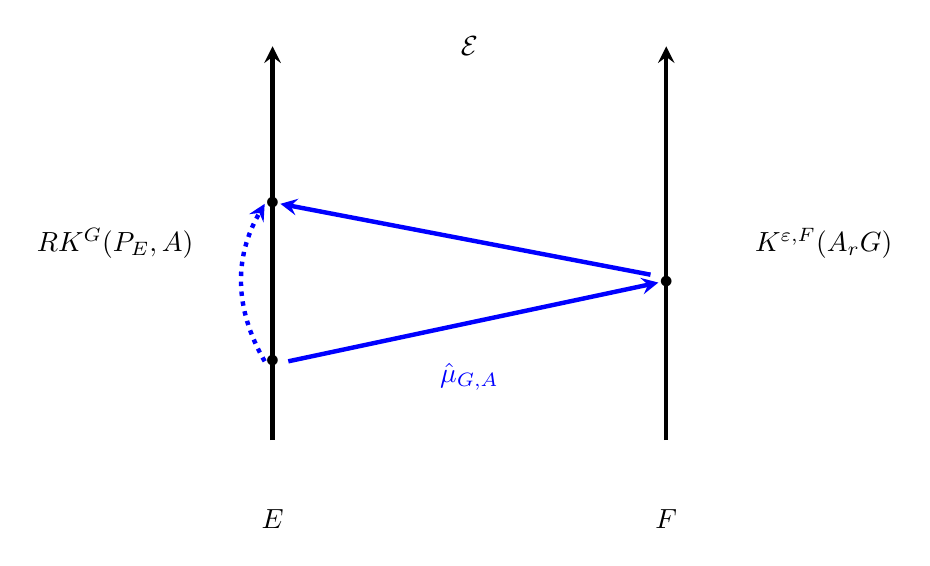
\begin{tikzpicture}
\draw  (2.5,5) node {$\mathcal E$};
\draw  (0,-1) node {$E$};
\draw  (5,-1) node {$F$};
\draw  (-2,2.5) node {$RK^G(P_E,A)$};
\draw  (7,2.5) node {$K^{\varepsilon,F}(A\rtimes_r G)$};
\draw [>=stealth, ->,ultra thick] (0,0) -- (0,5) ; %->
\draw [>=stealth, ->,ultra thick] (5,0) -- (5,5) ; 

\pause
\draw  (0,1) node {$\bullet$};
\draw  (5,2) node {$\bullet$};
\draw [>=stealth, ->,ultra thick, blue] (0.2,1) -- (4.9,2) ; 
\draw[blue] (2.5,0.8) node {$\hat\mu_{G,A}$};

\pause
\draw  (0,3) node {$\bullet$};
\draw [>=stealth, ->,ultra thick, blue] (4.8,2.1) -- (0.1,3) ; 

\pause
\draw [>=stealth, ->,ultra thick, blue, dotted] (-0.1,1) to[bend left] (-0.1,3) ; 

\end{tikzpicture}\]
\end{frame}





















%Unfinished ideas
%\section{Decomposition complexity}

Let $G$ be an étale groupoid with a proper length $l$. Fix $s>0$, and $G_s=\{g\in G : l^{r(g)}(g)\leq s\}$. For each subset $U$ of $X$, we can define the $s$-neiborghood of $U$ :
\[U_s = \{x\in X : \exists g\in G_s \text{ s.t. } r(g)\in U \text{ and } s(g)=x \}.\]

\begin{definition}
Let $G$ be an étale groupoid with compact base space $X$, and $\mathcal F$ a family of groupoids . We say that $G$ decomposes over $\mathcal F$ if, for every $R>0$, there exists a decomposition $X=X^{(1)}\cup X^{(2)}$ into subspaces such that each subspace $X^{(i)}$ is a disjoint union $\sqcup_j X^{(i)}_j$ satisfying the following conditions :
\begin{itemize}
\item[$\bullet$] if $j\neq j'$,  $X^{(i)}_{j,R}\cap X^{(i)}_{j'}=\varnothing$
\item[$\bullet$] there exists $s>0$ such that for every $i,j$, the groupoid $G_{j,s}^{(i)}$ generated by $G_{|X^{(i)}_j}\cap G_s$ is relatively compact and is in $\mathcal F$.
\end{itemize}
\end{definition}

\subsection{Examples and applications}

\begin{itemize}
\item[$\bullet$] \textbf{Motivating example.} Let $G=G(X)$ the coarse groupoid associated to a uniformly discrete metric space $X$ with bounded geometry. Then $G$ has FDC iff $X$ has FDC.\\
\item[$\bullet$] \textbf{Dynamic asymptotic dimension.} Recall that an étale groupoid is said to have dynamic asymptotic dimension $d$ if it is the smallest integer such that for every relatively compact subset $K$ of $G$, there exist open subsets $U_0$, ...,$U_d$ of $G^{(0)}$ such that they cover $r(K)\cup s(K)$ and for each $j$, $G_{|U_j}\cap K$ generates a relatively compact subgroupoids of $G$. Then if $G$ has finite dynamic asymptotic dimension, it has FDC. 

\item[$\bullet$] \textbf{Nuclear dimension :} Obtaining a bound on $\dim_{nuc}(A\rtimes G)$ w.r.t. $\dim_{nuc} (A\rtimes G_1)$ and $\dim_{nuc} (A\rtimes G_2)$, maybe $\dim_{cov}(G^{(0)})$.
\item[$\bullet$] \textbf{Mayer Vietoris :} $A\rtimes G_1$ and $A\rtimes G_1$ are a coercive pair, and we have quantitative Mayer-Vietoris. 
\end{itemize}





%\section{ Mayer-Vietoris exact sequences and controlled cutting and pasting}

\subsection{Mayer-Vietoris sequence in $K$-homology}

We first recall how to construct a Mayer-Vietoris element out of any pull back diagram of $C^*$-algebras.\\

Let us decompose $X$ into two open sets $U_0$ and $U_1$ and consider the $C^*$-algebras $A=C_0(X)$, $A_j=C_0(U_j)$ where $U_{01}=U_0\cap U_1$, and the cone $C$ of $A_0\oplus A_1$, with the canonical morphisms $\alpha :C \rightarrow A$ and $\beta : C \rightarrow SA_{01}$. The first is an homotopy equivalence, and the Mayer-Vietoris boundary is defined as the dotted arrow in the following commutative diagram
\[\begin{tikzcd}
KK^G_*(C,B) \arrow{r}{\beta^*}\arrow{d}{ \alpha^*}& KK^G_*(SA_{01},B)\arrow{d}{[\partial_{A_{01}}]\otimes -}\\
KK^G_*(A,B) \arrow[dotted]{r}& KK^G_{*+1}(A_{01},B)\\
\end{tikzcd}\]

where the right vertical arrow is the Bott element $[\partial_{A_{01}}]\in KK_1^G(A_{01},SA_{01})$.\\

At the level of controlled $K$-theory, Oyono-Oyono and Yu introduced a notion of Mayer-Vietoris pair in a filtered $C^*$-algebra $A$ weaker than that of a pull-back diagram. Recall that a $R$-controlled weak Mayer-Vietoris pair for $A$ is a quadruple $(\Delta_0,\Delta_1,A_0,A_1)$ such that for some constant $c$:\\

\begin{itemize}
\item[$\bullet$] if $x\in M_n(A_s)$ for $s\leq R$ and any $n>0$ , there exists $x_j\in M_n(\Delta_j\cap A_s)$ such that $x=x_0+x_1$ and $||x_j||\leq c||x||$,
\item[$\bullet$] $A_j$ is filtered by $(A_j\cap A_s)_{s\geq 0}$ and $C^* N_{\Delta_j}^{(R,5R)}\subset A_j$
\item[$\bullet$] for any $\epsilon >0$, if $x\in M_n(A_{0,s})$, $y\in M_n(A_{1,s})$ such that $||x-y||<\epsilon$,  there exists $z\in M_n(A_{0,s}\cap A_{1,s})$ with $||z-x||<\epsilon$ and $||z-y||<\epsilon$. \\
\end{itemize}

For example, take $G$ to be an étale groupoïd with proper length $l$, with compact base space $X$. The convolution algebra $C^*_r G$ is filtered by $(C_c(G_R))_{R>0}$, $G_R=l^{-1}[0,R)$. Fix $R>5r$. If $V$ is an open subset of $X$, set \\

\begin{itemize}
\item[$\bullet$] $V^R= \{r(g) : g\in G_V\cap G_R\}$,
\item[$\bullet$] $\Delta_V = C_0(G_V\cap G_R)$
\item[$\bullet$] $G_{V,R}^V = \langle G_V^V \cap G_R \rangle$\\
\end{itemize} 

then $(\Delta_{V_0},\Delta_{V_1}, C_r^*(G_0),C_r^*(G_1))$ is a $r$-controlled Mayer-Vietoris pair for $C^*_r G$ when $X=V_0\cup V_1$, and $G_j = G_{V_j^R}^{V_j^R , (R)}$.\\

The existence of a controlled Mayer-Vietoris pair is nice, because even if the $C^*$-algebra is simple, it can possess such a decomposition, and the following result gives a way to compute the $K$-theory analogous to the situation of a classical Mayer-Vietoris decomposition :

\begin{thm}
For every positive $c$, there exists a control pair $(\lambda,h)$ such that for any filtered $C^*$-algebra $A$ which has a $R$-controlled Mayer-Vietoris pair $(\Delta_0,\Delta_1,A_0,A_1)$ the following sequence is $(\lambda,h)$-exact at order $R$
\[\begin{tikzcd}
\hat K_0(A_0\cap A_1 ) \arrow{r}& \hat K_0(A_0)\arrow{r}\oplus \hat K_0(A_1) & \hat K_0(A)\arrow{d}{D} \\
\arrow{u}{D}\hat K_1(A) &\arrow{l} \hat K_1(A_0)\oplus \hat K_1(A_1) & \arrow{l}\hat K_1(A_0\cap A_1) 
\end{tikzcd}\]
where $D$ is a controlled Mayer-Vietoris boundary.\\
\end{thm}

To go back to our example, if $X=V_0\cup V_1$, we simulteanously have two decompositions : that arising from the decomposition of the Rips simplex into two open sets $P_d(G^{V^R,(R)}_{V^R})$, and that of the controlled Mayer Vietoris pair. The aim of this section is to show that the quantitative assembly maps respects these two exact sequences in a precise way.\\

Actually, in this particular case, the quantitative Mayer-Vietoris exact sequence should hold at all orders, which would allows us to state a much stronger result, with more interesting applications : a Künneth formula for crossed product algebras of étale groupoids.\\

\textbf{A remark :} There is a seemingly harmful parallel between the controlled Mayer-Vietoris decomposition and the nuclear dimension of the reduced $C^*$-algebra. Namely, to show that the pair satisfies the Mayer-Vietoris conditions, we make use of the completely positive map induced by 
\[\left\{\begin{array}{lcr} C_c(G) &\rightarrow & C_c(G) \\ f &\mapsto & \phi_0\circ r\ . f .\ \phi_0\circ s\end{array}\right.\]   
where $\phi_0$ is any continuous function $X\rightarrow [0,1]$ with support in $V_0$ which is $1$ on some compact $K\subset V_0$.\\
Could we push the analogy further ? 

\subsection{Standard modules}

The aim of this section is to develop a notion of non-degenerate standard modules over a groupoid analogous to non-degenerate standard modules over coarse spaces. \\

Let us first recall the coarse case. Let $X$ be a discrete metric space with bounded geometry. 

\begin{definition}
A $X$-module is a Hilbert space $H_X$ equipped with a $*$-representation $\phi : C_0(X) \rightarrow \mathcal L(H_X)$. The $X$-module $(H_X,\phi)$ is said to be :\\

\begin{itemize}
\item[$\bullet$] standard if $\phi(C_0(X))H_X$ is dense in $H_X$,
\item[$\bullet$] non-degenerate if $\forall f \in C_0(X), \phi(f)\in \mathfrak K (H_X) \implies f=0$.
\end{itemize}
\end{definition}

The usefulness of n.d.s. $X$-modules comes from the following lemma :

\begin{lem}
Let $X$ and $Y$ be two discrete metric spaces with bounded geometry, and $h : X\rightarrow Y$ a coarse map. Then, for any two standard modules $H_X$ and $H_Y$ over $X$ and $Y$ respectively, there exists an isometry which covers $h$, i.e. for any $\epsilon >0$, there exists $V\in \mathcal L(H_X,H_Y)$ such that 
\[\text{supp }V \subset \{(x,y)\in X\times Y, d(h(x),y)<\epsilon\}.\]
\end{lem}

\textbf{Remark :} We can induce $V$ on the Roe algebras by $\forall T\in C^*(X,H_X), Ad_V(T) := V T V^* \in C^*(Y,H_Y)$, and the preceding lemma entails that \[(Ad_V)_* : K(C^*(X,H_X))\rightarrow K(C^*(Y,H_Y))\] only depends on the coarse class of $h$. We directly see that the $K$-theory of the Roe-algebras of $X$ do not depend on the standard modules if they are n.d.s. : one just need to take an isometry covering the identity. \\

We can actually show that taking the Roe algebra is a functor. Choose, for any coarse space $X$ a n.d.s. $X$-module $H_X$, and consider the category $Coarse$ of coarse spaces with morphisms coarse maps, and the category $KK$ with objects $C^*$-algebras, and morphisms defined by $KK$-theory, $Hom_{KK}(A,B)=KK(A,B)$. Then $ X \mapsto C^*(X,H_X) $ and $\left(h:X \rightarrow Y\right) \mapsto (Ad_V)_*\in KK(C^*(X,H_X),C^*(Y,H_Y))$ defines a functor $Coarse \rightarrow KK$, which does not depend on the choices $X\mapsto H_X$ being made.\\

We will focus ont the following result :

\begin{thm}
Let $X$ be a finite simplicial complex, and $B$ a $C^*$-algebra. There exists $\varepsilon_0\in (0,\frac{1}{4})$ such that for all $\varepsilon \in (0,\varepsilon_0)$, there exists $R_\varepsilon>0 $ s.t. 
\[\forall R\in (0,R_\varepsilon),\  Ind_{X,B}^{\varepsilon, R} : KK(C(X),B)\rightarrow K^{\varepsilon,R}(B\otimes \mathfrak K(H_X))\] 
is an isomorphism.
\end{thm}

We wish to prove a similar result for "nice" groupoids. Let us recall the definition of $G$-simplicial complex from \ref{TuBC2}.

\begin{definition}
Let $G$ be a locally compact groupoid. A $G$-simplicial complex of dimension less than $n$ is a triple $(Z,\Delta, p)$ where
\begin{itemize}
\item[$\bullet$] $Z$ is a locally compact space of vertices and $p: Z \rightarrow G^{(0)}$ a locally injective map, which is an anchor map for an action of $G$, 
\item[$\bullet$] $\Delta$ is a closed $G$-invariant subset of the probability measures $P(Z)$ on $Z$, equipped with the weak-$*$ topology, with the property that every element of $\Delta$ has a support contained in a fiber of $p$ and has at most $n+1$ elements. Such a support is call a simplex of $\Delta$. Moreover, if $\nu\in \Delta,\mu \in P(Z)$ and $supp(\mu)\subset supp(\nu)$ then $\mu\in \Delta$.
\end{itemize}
\end{definition}

The first step is to defined what is a s.n.d. $G$-module.

\begin{definition}
A s.n.d. $G$-module is a triple $(E,\phi,V)$ where $E$ is a $C_0(G^{(0)})$-algebra, $\phi : C_0(G^{(0)})\rightarrow \mathcal L(E)$ is a $*$-representation and $V$ is an action of $G$ on $E$ such that
\begin{itemize}
\item[$\bullet$] $E$ decomposes as a external tensor product $E\simeq E^{(0)}\otimes E^{(1)}$ of $G$-modules such that there exists $\phi : C_0(G^{(0)})\rightarrow \mathcal L(E^{(0)})$ and $\phi= \phi_0\otimes id_{E^{(1)}}$
\item[$\bullet$] No non-zero function of $C_0(G^{(0)})$ acts as a compact operator via $\phi_0$, and $\overline{\phi_0(C_0(G^{(0)}))E^{(0)} }= E^{(0)}$
\item[$\bullet$] For all compact subgroupoids $K$ of $G$, there exists an isomorphism of $K$-modules $\text{Res}_K^G E^{(1)} \simeq L^2(K)\otimes H_K$ where $H_K$ is a separable Hilbert space.
\end{itemize}
\end{definition}

Now we want to show the following :

\begin{lem}
Let $G$ be a locally compactly induced groupoid, and $E,E'$ any two s.n.d. $G$-modules, then for any compact subset $K$ of $G$, there exists an isometry $V\in \mathcal L(E,E')$ such that 
\[supp\ V \subset (s\times r)(K). \]
\end{lem}

\begin{dem}
Let $E$ a n.d.s. $G$-module, and decompose the base space $G^{(0)}$ into $G$-invariant subset which are locally induced by compact subgroupoids of $G$ :
\[G^{(0)} = \cup_{j=1}^J G\times_{K_j} U_j.\]
By the third hypothesis of being s.n.d., there exist a Hilbert space $H_j$ and an isomorphism of Hilbert modules $F_j :\text{Res}_{K_j}^G E^{(1)} \rightarrow  L^2(K_j)\otimes H_j$, but the induction $\text{Ind}_{K_j}^G L^2(G/K_j)\otimes L^2(K_j)\otimes H_j$ is non canonically isomorphic to $L^2(G)\otimes H_j$, so that $E$ is isomorphic to $E^{(0)}\otimes L^2(G)\otimes H_j$.\\
\qed
\end{dem}

\begin{cor}
Let $G$ and $G'$ two locally compactly induced groupoids, $E,E'$ two s.n.d. modules over $G$ and $G'$ respectively and $(Z,p,p')$ a generalized morphism from $G$ to $G'$ which respects condition ??. For any compact subset $K$, there exists an isometry $V\in \mathcal L(E,E')$ such that
\[supp\ V \subset (p\circ (p')^{-1}(s(K))\times r)(K). \]
\end{cor}
























 



%\section{Nuclear dimension}

In their paper \cite{GWY}, E. Guentner, R. Willett and G. Yu defined asymptotic dimension for étale groupoids, and the theorem which we are intersted in is the following.

\begin{thm}
Let $G$ be an étale groupoid with finite asymptotic dimension, and with base space $G^{(0)}$ of finite covering dimension. If $G$ is free, then the following inequality holds :
\[\text{dim}^{+1}_{nuc}(C^*_rG)\leq \text{dim}^{+1}_{cov}(G^{(0)}).\text{asdim}^{+1}(G).\] 
\end{thm}

The article points out that freeness is mainly technical, and that one could somehow could get rid of it. That is what we entail to do. \\

The point of the proof is to construct, out of any compact subset $K\subset G$, an almost invariant partition of unity subordinate to a covering fulfilling the definition of asymptotic dimension. This PDU is use to construct a completely positive factorisation of the identity of $C^*_rG$ through the reduced $C^*$-algebra of the open relatively compact subgroupoids generated by restiction to the cover and intersection with $K$. Here freeness does not intervene. \textbf{VERIFY} \\

Freeness is only used for this paticular result.

\begin{prop}
Let $G$ a free étale groupoid, and $H$ an open relatively compact subgroupoid of $G$. Then 
\[\text{dim}_{nuc} C^*_r H = \text{dim}_{cov} H^{(0)}.\]
\end{prop}

Of course, the result should not hold without any assumption on $G$, more precisely, I think we should ask something about the isotropy bundle of $G$.\\

\begin{definition}
The isotropy bundle of $G$ is the closed subgroupoid $\mathcal J = (r\times s)^{-1}(\Delta)$, i.e. the group bundle of the stabilizers $\mathcal J = \cup G_x^x$. Here $\Delta\subset G^{(0)}\times G^{(0)}$ is the diagonal of the base space. 
\end{definition}

\textbf{Remark :} If $G$ is a (locally compact) transitive groupoid, then P. Muhly, J. Renault and D. Williams \textbf{ref !} have shown that $C^*_rG$ is isomorphic to $C^*_r H \otimes \mathfrak K(L^2(\mu))$ for $H$ any of the group statbilizers, which are all isomorphic, and $\mu$ a measure on $G^{(0)}$, so that
\[\text{dim}_{nuc}^{+1}(C_r^*G)\leq \text{dim}_{nuc}^{+1}(C_r^*H).\text{dim}_{nuc}^{+1}(\mathfrak K(L^2(\mu))).\]
by Prop. $2.3$ of \textbf{WZ}.

Let $H^{(0)}/H$ be the base space quotiented by the equivalence relation induced by $H$, and let $[x]=r(s^{-1}(x))$ denotes the equivalence class of $x\in H^{(0)}$, $\pi : H^{(0)}\rightarrow H^{(0)}/H$ the canonical projection map.\\  

\begin{prop}
Let $H$ be a compact étale groupoid. Then $X=H^{(0)}/H$ is compact and Hausdorff, moreover there exists a structure of $C(X)$-algebra on $C^*_rH$ with fibers isomorphic to $C^*_r(H_x^x)\otimes \mathfrak K(l^2([x]))$ for any $x\in H^{(0)}$.
\end{prop}

\begin{proof}
Define
\[\left\{\begin{array}{rcl} C(X) &\rightarrow & Z(\mathcal M(C^*_r H)) \\ f &\mapsto & f\circ \pi \end{array}\right. ,\]
which defines a $C(X)$-structure on $C^*_rH$.\\
Its fiber over $t\in X$ is given by the quotient by the ideal $C(H^{(0)}- t) C^*_r H $ i.e. $C^* H(t)$, as $H^{(0)}-t$ is an open $H$-invariant subset. But $H(t)$ is a principal groupoid so we can apply the remark to get $C^*_r H(t)\simeq C^*_r H_x^x \otimes \mathfrak K(l^2(t))$ where $x$ is any point of $t$.\\
\end{proof}

\begin{prop}
Let $H$ be a compact étale groupoid. \\
If, for all $x\in H^{(0)}$, $C^*_rH_x^x$ is a nuclear $C^*$-algebra, then $C^*_r H$ is nuclear.\\
If $\sup_{x\in H^{(0)}}\text{dim}_{nuc}(C^*_rH_x^x)\leq d$ then
\[\text{dim}_{nuc}(C^*_r H)\leq (\text{dim}_{cov}(H^{(0)})+1)(d+1)-1. \]
\end{prop}

\begin{proof}
\textbf{LATER}
\end{proof}









\bibliographystyle{plain}
\bibliography{biblio2} 
%\nocite{*}

\end{document}


























